%% Proyecto.tex
%% 2020/06/08
%% por Juan Pablo Mora
%% 
%% Proyecto que demuestra soluciones graficadas numéricamente para la
%% ecuación de Laplace
%%

\documentclass[10pt,journal,compsoc]{IEEEtran}

\ifCLASSOPTIONcompsoc
  % IEEE Computer Society needs nocompress option
  % requires cite.sty v4.0 or later (November 2003)
  \usepackage[nocompress]{cite}
\else
  % normal IEEE
  \usepackage{cite}
\fi

\usepackage{listings}
\usepackage{cancel}


\usepackage[pdftex]{graphicx}
% declare the path(s) where your graphic files are
\graphicspath{images/}
% and their extensions so you won't have to specify these with
% every instance of \includegraphics
\DeclareGraphicsExtensions{.png}

\usepackage{amsmath}
% A popular package from the American Mathematical Society that provides
% many useful and powerful commands for dealing with mathematics.
%
% Note that the amsmath package sets \interdisplaylinepenalty to 10000
% thus preventing page breaks from occurring within multiline equations. Use:
\interdisplaylinepenalty=2500
% after loading amsmath to restore such page breaks as IEEEtran.cls normally
% does. amsmath.sty is already installed on most LaTeX systems. The latest
% version and documentation can be obtained at:
% http://www.ctan.org/pkg/amsmath

% correct bad hyphenation here
\hyphenation{op-tical net-works semi-conduc-tor}


\begin{document}
%
% paper title
% Titles are generally capitalized except for words such as a, an, and, as,
% at, but, by, for, in, nor, of, on, or, the, to and up, which are usually
% not capitalized unless they are the first or last word of the title.
% Linebreaks \\ can be used within to get better formatting as desired.
% Do not put math or special symbols in the title.
\title{Soluciones de la Ecuación de Laplace}


\author{Juan~Pablo~Mora,~\IEEEmembership{Estudiante,~UVG}% <-this % stops a space
\IEEEcompsocitemizethanks{\IEEEcompsocthanksitem Thanks to Mr. Siba Prasad for all his help
during the course.}}

% The paper headers
\markboth{Teoría Electromagnética Sección~20, Proyecto~1, Mayo~2020}%
{Soluciones de la Ecuación de Laplace}
% The only time the second header will appear is for the odd numbered pages
% after the title page when using the twoside option.
% 
% *** Note that you probably will NOT want to include the author's ***
% *** name in the headers of peer review papers.                   ***
% You can use \ifCLASSOPTIONpeerreview for conditional compilation here if
% you desire.

\IEEEtitleabstractindextext{%
\begin{abstract}
Soluciones numéricas a la Ecuación de Laplace
\end{abstract}

% Note that keywords are not normally used for peerreview papers.
\begin{IEEEkeywords}
IEEE, IEEEtran, journal, \LaTeX, paper, Laplace equations.
\end{IEEEkeywords}}


% make the title area
\maketitle


% To allow for easy dual compilation without having to reenter the
% abstract/keywords data, the \IEEEtitleabstractindextext text will
% not be used in maketitle, but will appear (i.e., to be "transported")
% here as \IEEEdisplaynontitleabstractindextext when the compsoc 
% or transmag modes are not selected <OR> if conference mode is selected 
% - because all conference papers position the abstract like regular
% papers do.
\IEEEdisplaynontitleabstractindextext
% \IEEEdisplaynontitleabstractindextext has no effect when using
% compsoc or transmag under a non-conference mode.



% For peer review papers, you can put extra information on the cover
% page as needed:
% \ifCLASSOPTIONpeerreview
% \begin{center} \bfseries EDICS Category: 3-BBND \end{center}
% \fi
%
% For peerreview papers, this IEEEtran command inserts a page break and
% creates the second title. It will be ignored for other modes.
\IEEEpeerreviewmaketitle



\IEEEraisesectionheading{\section{Introducción}\label{sec:introduction}}
% Computer Society journal (but not conference!) papers do something unusual
% with the very first section heading (almost always called "Introduction").
% They place it ABOVE the main text! IEEEtran.cls does not automatically do
% this for you, but you can achieve this effect with the provided
% \IEEEraisesectionheading{} command. Note the need to keep any \label that
% is to refer to the section immediately after \section in the above as
% \IEEEraisesectionheading puts \section within a raised box.




% The very first letter is a 2 line initial drop letter followed
% by the rest of the first word in caps (small caps for compsoc).
% 
% form to use if the first word consists of a single letter:
% \IEEEPARstart{A}{demo} file is ....
% 
% form to use if you need the single drop letter followed by
% normal text (unknown if ever used by the IEEE):
% \IEEEPARstart{A}{}demo file is ....
% 
% Some journals put the first two words in caps:
% \IEEEPARstart{T}{his demo} file is ....
% 
% Here we have the typical use of a "T" for an initial drop letter
% and "HIS" in caps to complete the first word.
\IEEEPARstart{E}{l} objetivo de este articulo es demostrar el comportamiento
de potenciales eléctricos resolviendo la Ecuación de Laplace con condiciones de
frontera de Dirichlet.
\\\\
El documento consiste en los ejercicios asignados y su respectiva solución,
la cual será mostrada como un grafico en 3D o un mapa de calor en 2D el cual se
calcula utilizando el método analítico y el "truco de Fourier" para la resolución
de ecuaciónes diferenciales parciales.
\\\\
Adicionalmente en el apéndice A se escribe sobre el método de resolución y sobre 
las formas alternativas con las que se puede calular la misma solución.
\hfill mds
 
\hfill Junio 7, 2020

\subsection{Ecuación de Laplace en coordenadas rectangulares}

\subsubsection{Tubería rectangular}
Una tubería rectangular recta se extiende infinitamente a lo largo del eje \(z\).
Sus paredes se encuentran en los planos \(x=0,y=0,x=a\) y \(y=b\).
Los planos \(y = 0\) y \(y = b\) se encuentran aterrizados, mientras que los planos
\(x = 0\) y \(x = a\) se encuentran a potenciales \(g(y)\) y \(h(y)\) respectivamente.
\\\\
Determine el potencial eléctrico dentro dentro de la tubería bajo las siguientes condiciones:
\(g(y) = 0, h(y) = tan^{-1}(y/a)\)
\\

\subsubsection{Condiciones iniciales del problema}

Para empezar, escogemos un valor arbitrario para a y b, por simplicidad usamos \(a = b = 35 \)
y configuramos \(h(y) = tan^{-1}(y/a) \quad 0\leq y \leq a \)
el resultado del potencial y el campo vectorial en \(n = 20\) se puede ver en la grafica \ref{arctan-n20}
y las gráficas de menores iteraciones incluyendo las condiciones iniciales y la densidad de carga
se encuentran en la figura \ref{arctan-iterations}.

\subsubsection{Solución analítica}

La solución general de la Ecuación de Laplace es \(V(x,y)=(Ae^{kx}+B^{-kx})(C sin(ky) + D cos(ky))\)
Al utilizar las condiciones de frontera mencionadas antes podemos resolver
\begin{align*}
  V(x,y)&=(\cancelto{0}{A}e^{kx}+Be^{-kx})(C sin(ky) + D cos(ky))\\
  &\text{ Por x} \to \infty, V \to 0\\
  V(x,0)&=(Be^{-kx}) (\cancelto{0}{D}cos(ky)) = 0\\
  V(x,b)&=Ce^{-kx}sin(kb) = 0 \to k=\frac{n*\pi}{b}\\
  &\text{Esto nos da una lista de coeficientes de n:}\\
  C_{n} &e^{-\frac{xn*\pi}{b}} sin(\frac{yn\pi}{b}) \text{ y }\\
  V_o(y)&= \sum_{n=1}^{\infty} C_{n} e^{-\frac{xn*\pi}{b}} sin(\frac{yn\pi}{b})\\\\
  &\text{Con el "Truco de Fourier" simplificamos la ecuación}\\
  &\text{Usando la propiedad } \int_{0}^b  sin(\frac{yn\pi}{b}) sin(\frac{yn'\pi}{b})dy = \frac{b}{2}\\
  \int_{0}^b&V_o(y)sin(\frac{yn\pi}{b})dy=\\
  &=\sum_{n=1}^{\infty} C_{n} e^{-\frac{xn*\pi}{b}} \cancelto{\frac{b}{2}}{\int_{0}^b sin(\frac{yn\pi}{b}) sin(\frac{yn'\pi}{b})dy}\\
  \int_{0}^b&V_o(y)sin(\frac{yn\pi}{b})dy=\frac{2}{b} \sum_{n=1}^{\infty} C_{n} e^{-\frac{xn*\pi}{b}}\\
  &\text{Finalmente despejamos para \(C_n\)}\\
  C_n &= \frac{2}{b} sin(\frac{n\pi y}{b}) \int_0^b \tanh(\frac{y}{a})\sin(\frac{n\pi y}{b}) dy\\
  &\text{Reeplazamos en la ecuación original}\\
  V(x,y)&=\sum_{n=1}^{\infty} \frac{2}{b} sin(\frac{n\pi y}{b}) \int_0^b \tanh(\frac{y}{a})\sin(\frac{n\pi y}{b}) dy\\
\end{align*}

\subsubsection{Solución numérica}

Para configurar las condiciones iniciales en el código utilizamos
\begin{lstlisting}
  T[:,-1] = np.arctan(y/y[-1])
\end{lstlisting}

\begin{figure}
  \centering
  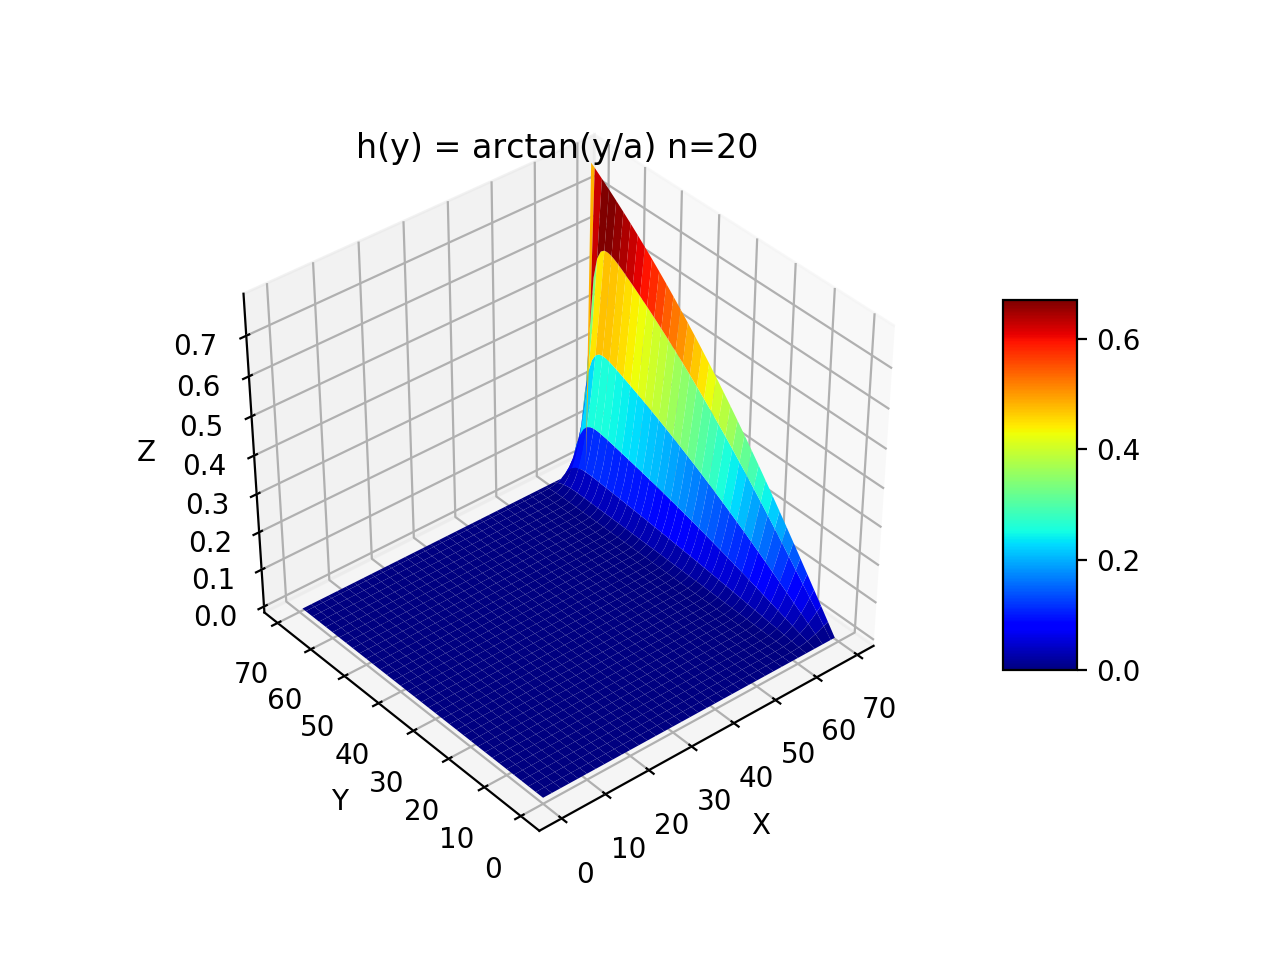
\includegraphics[width=2.8in]{images/arctan-n20}
  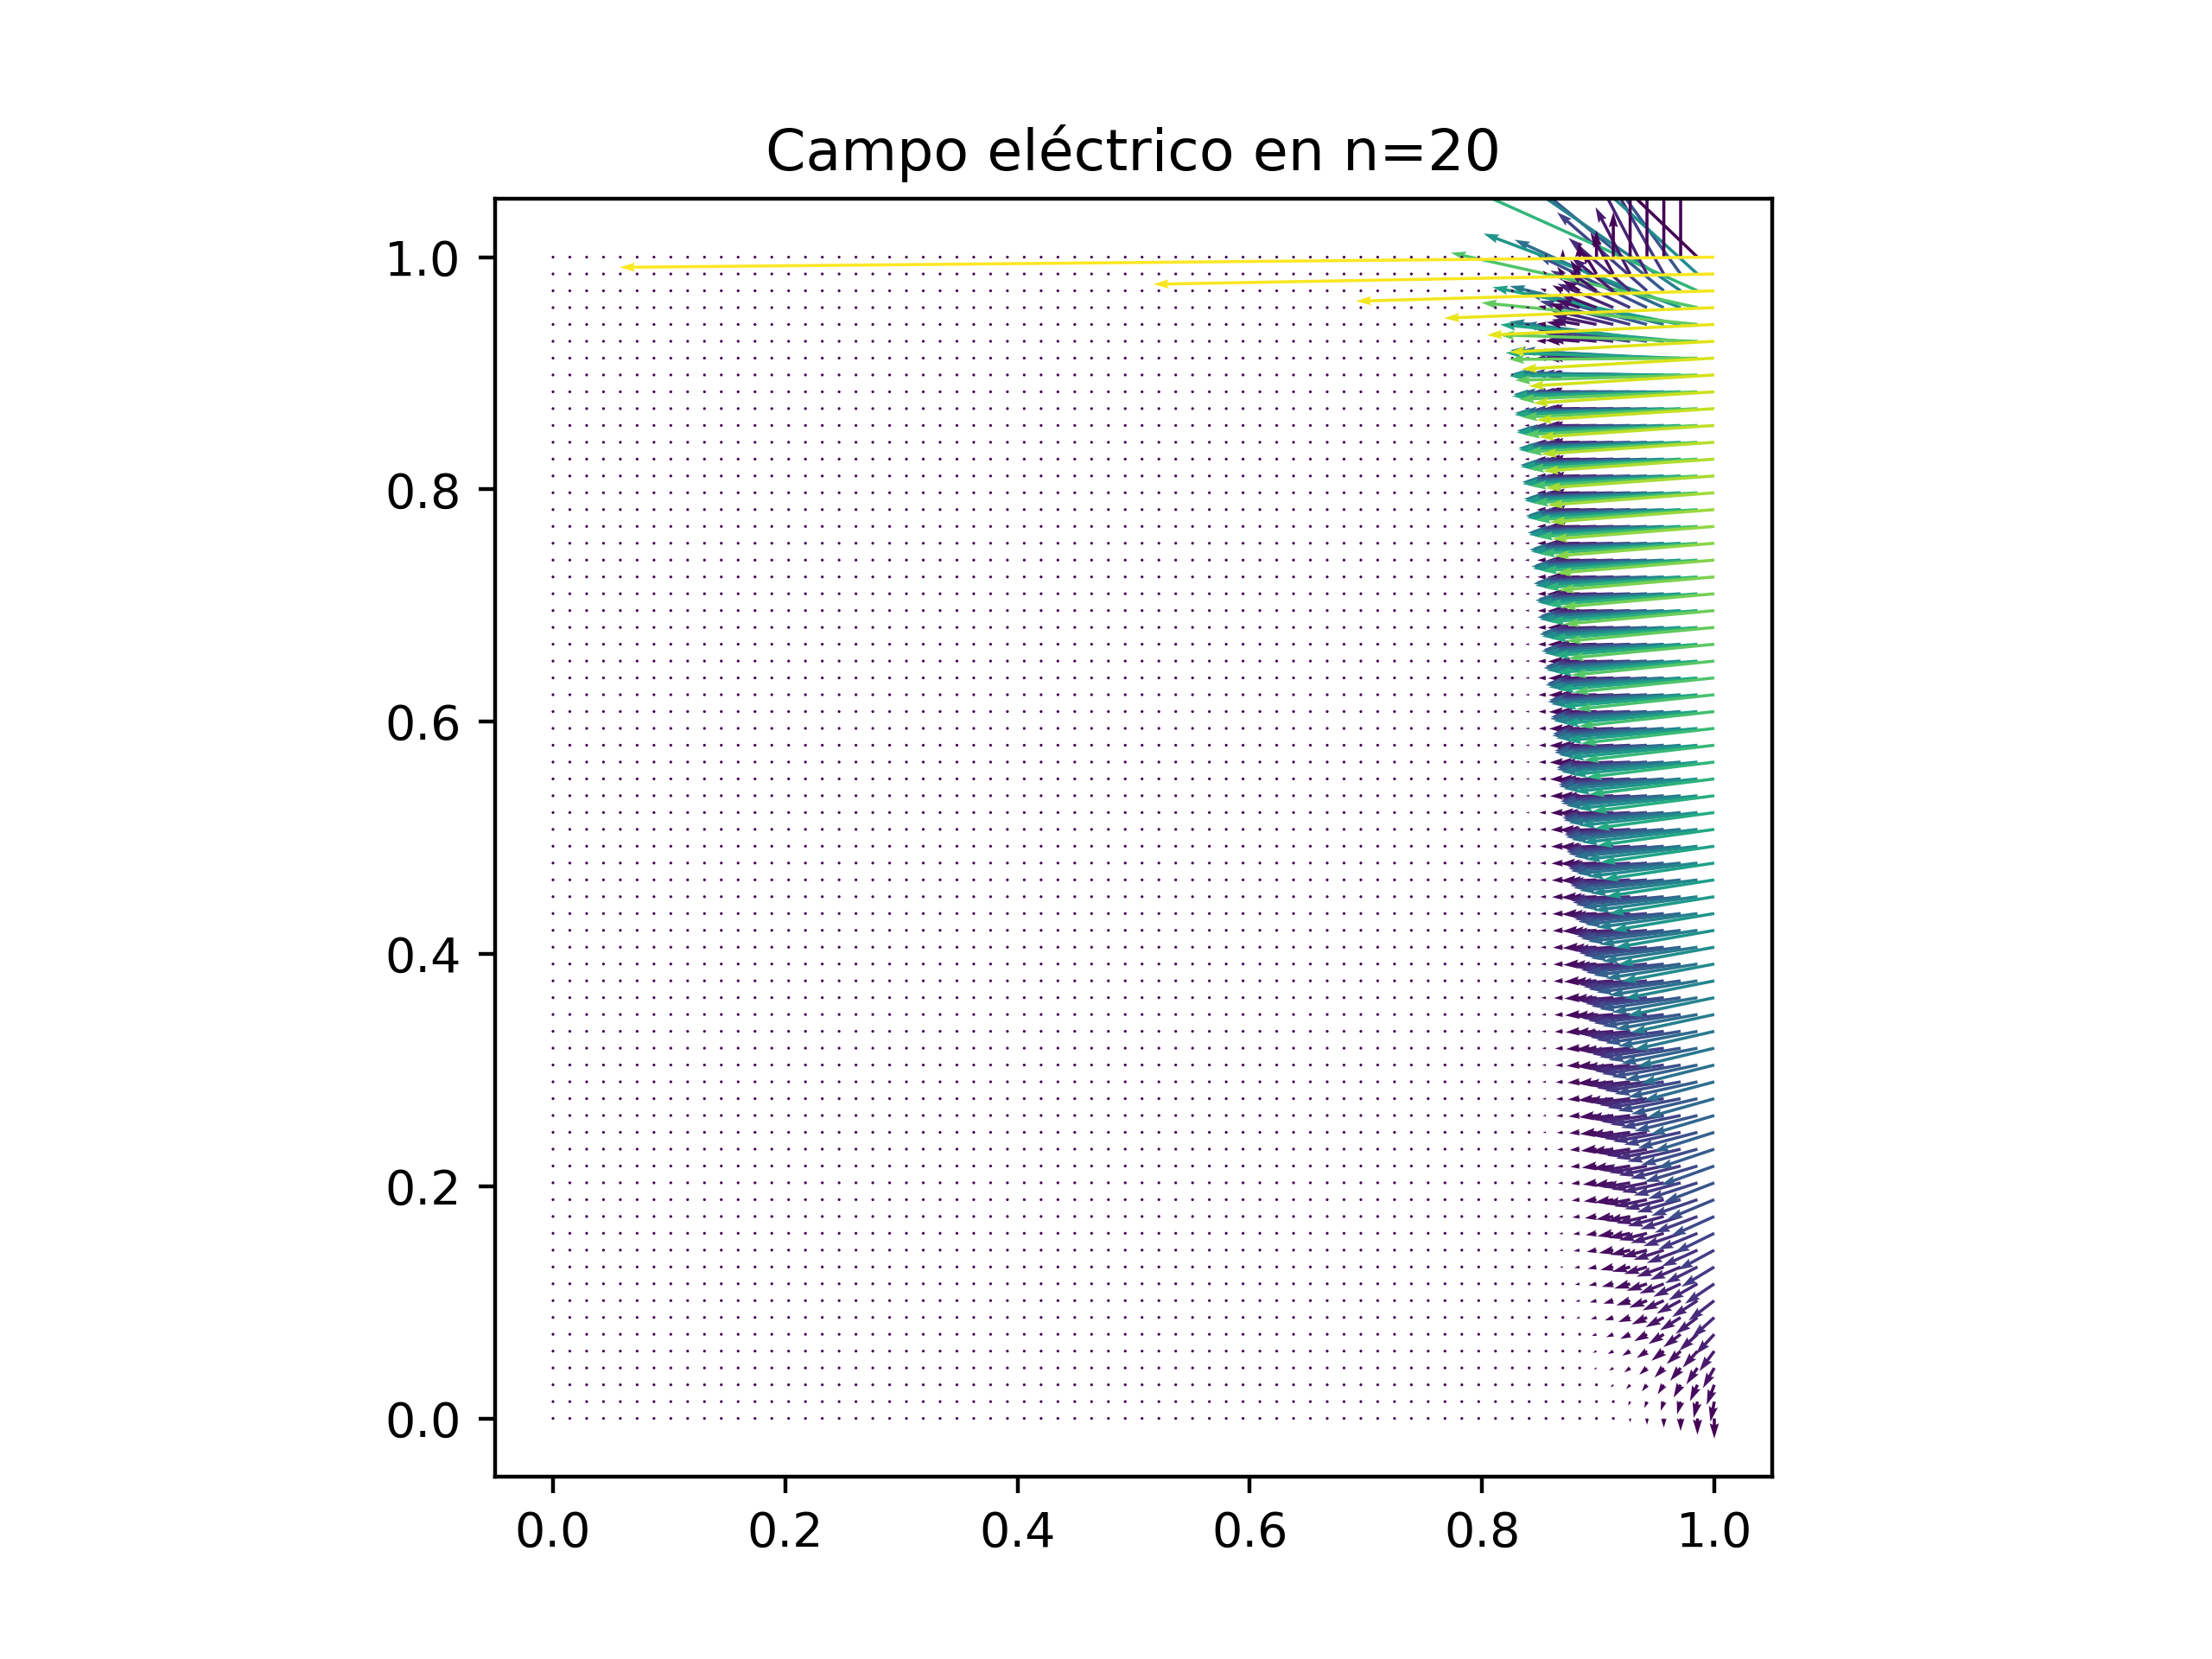
\includegraphics[width=2.8in]{images/arctan-field}
  \caption{Potencial y campo eléctrico para \(h(y) = tan^{-1}(y/a)\)}
  \label{arctan-n20}
\end{figure}

\begin{figure}
  \centering
  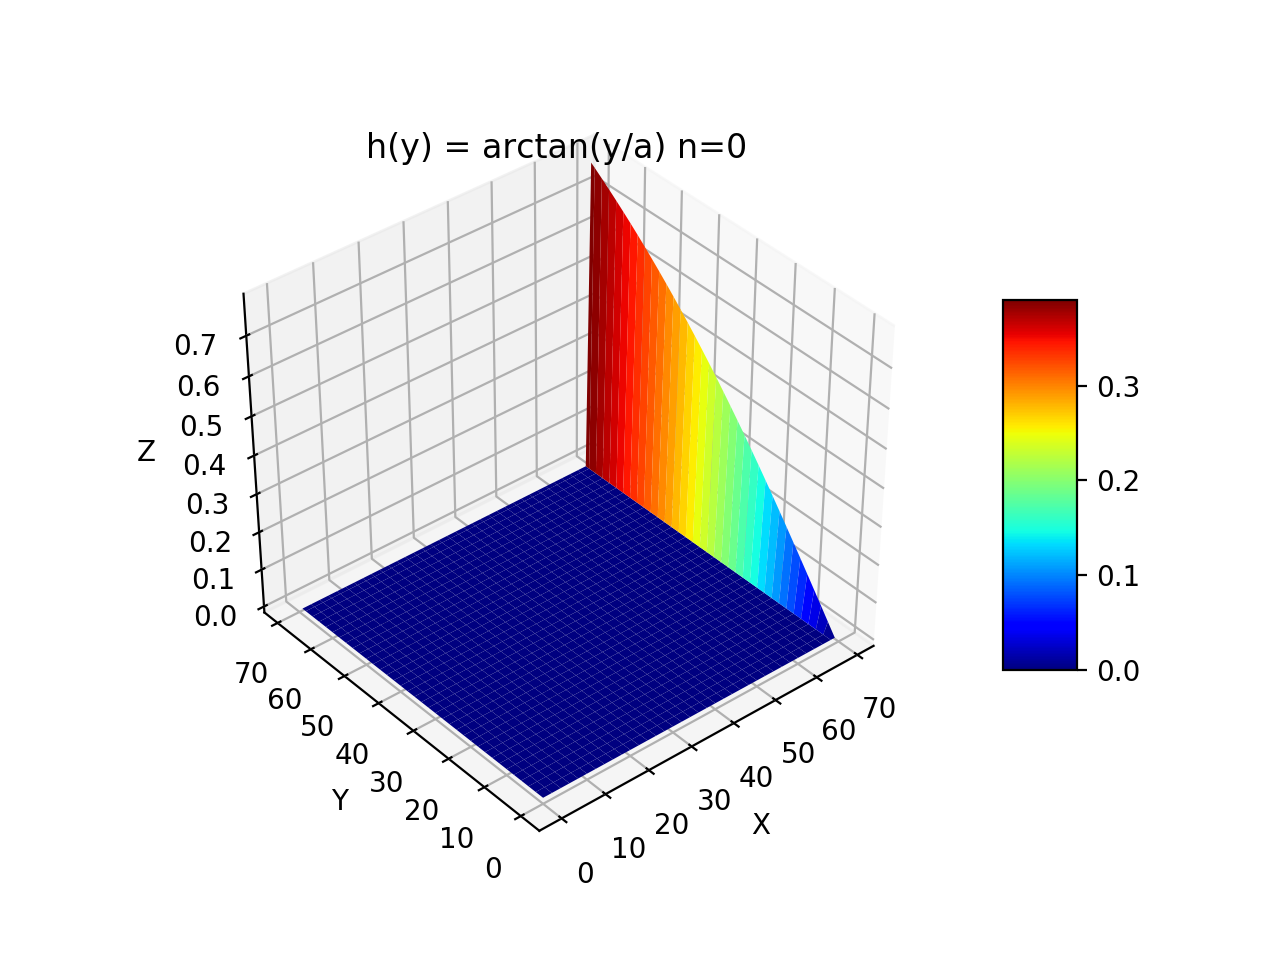
\includegraphics[width=1.5in]{images/arctan-n0}
  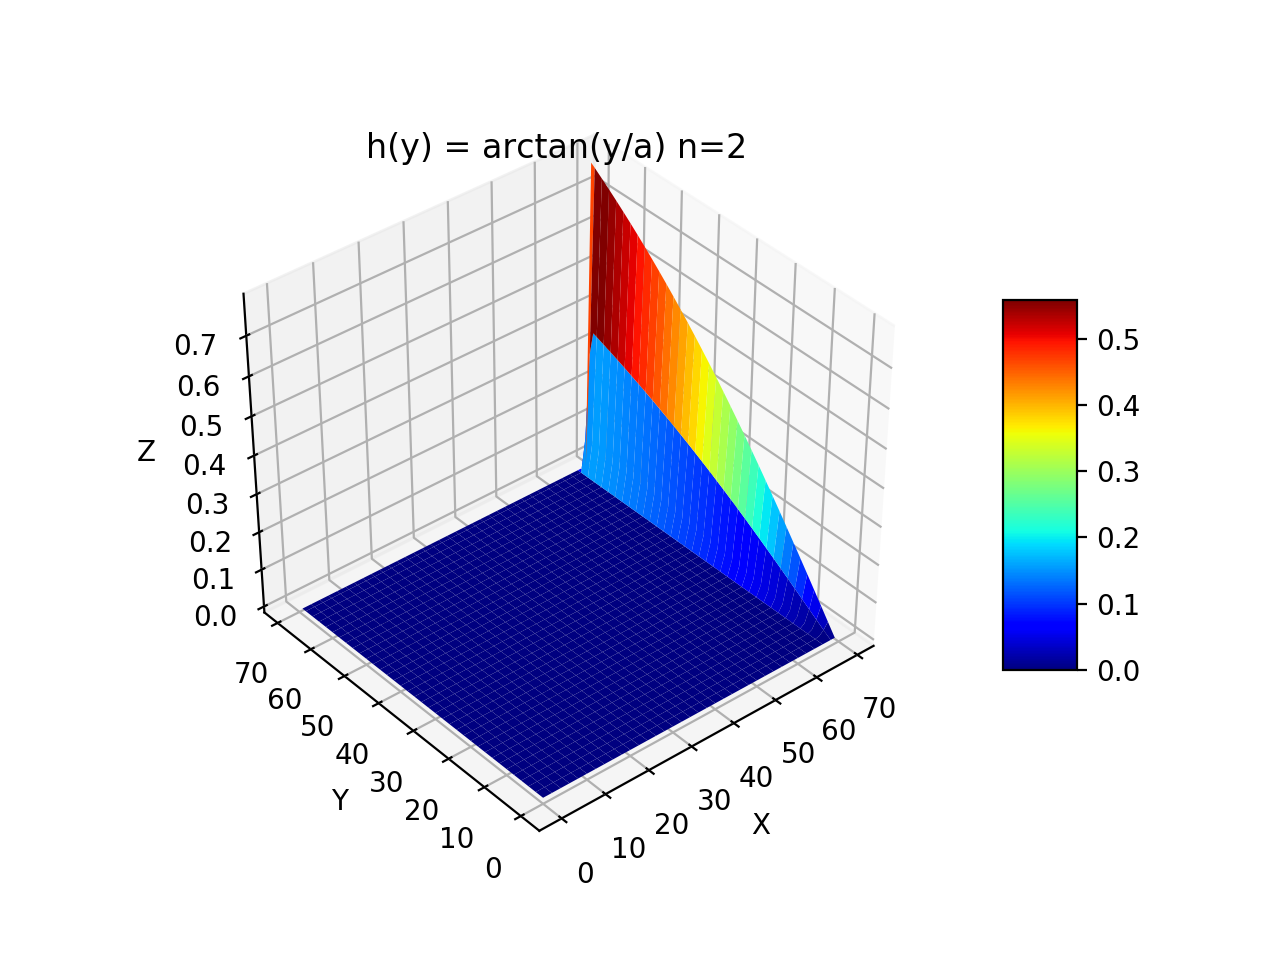
\includegraphics[width=1.5in]{images/arctan-n2}
  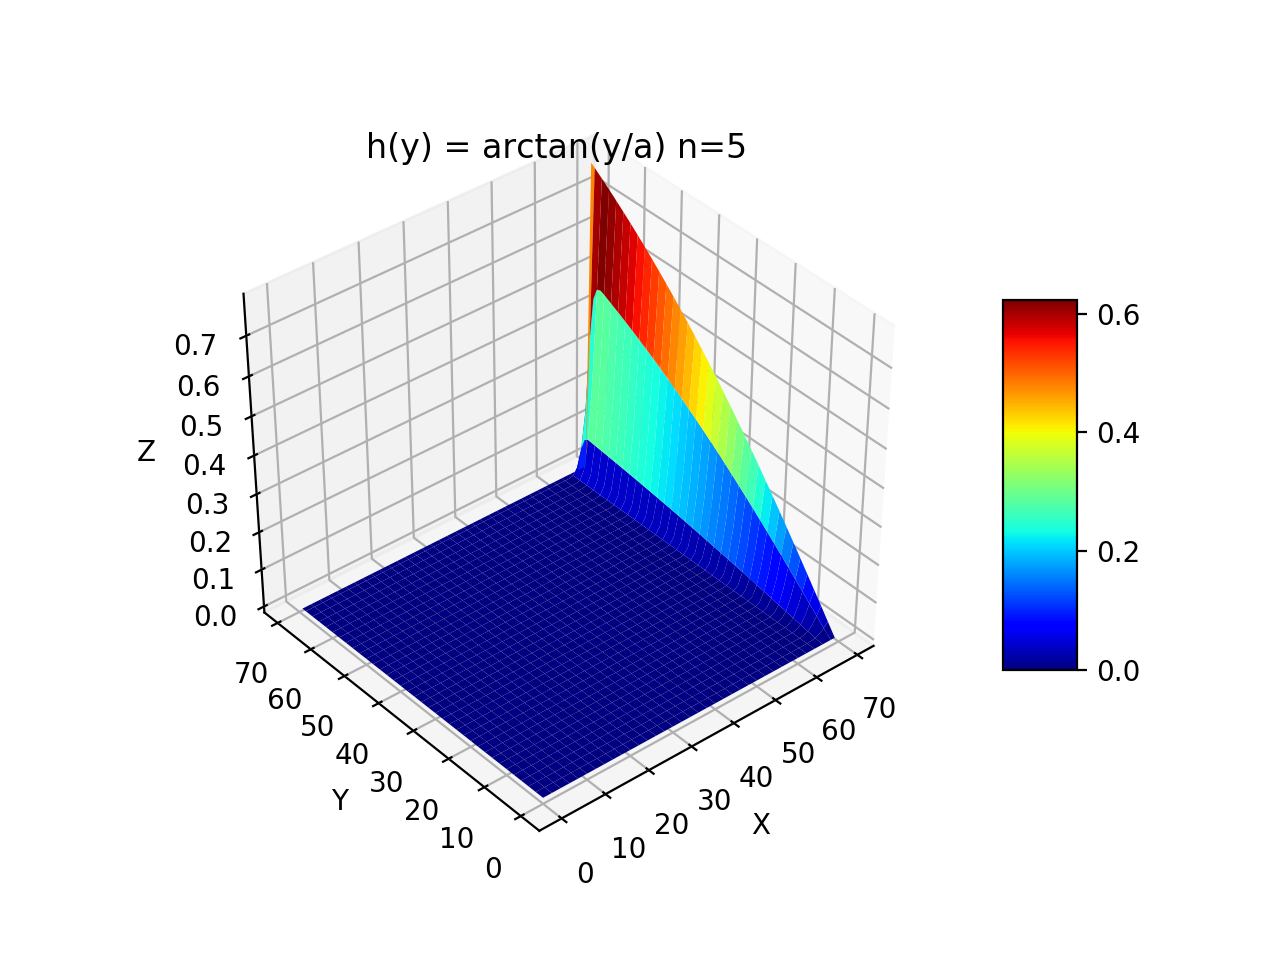
\includegraphics[width=1.5in]{images/arctan-n5}
  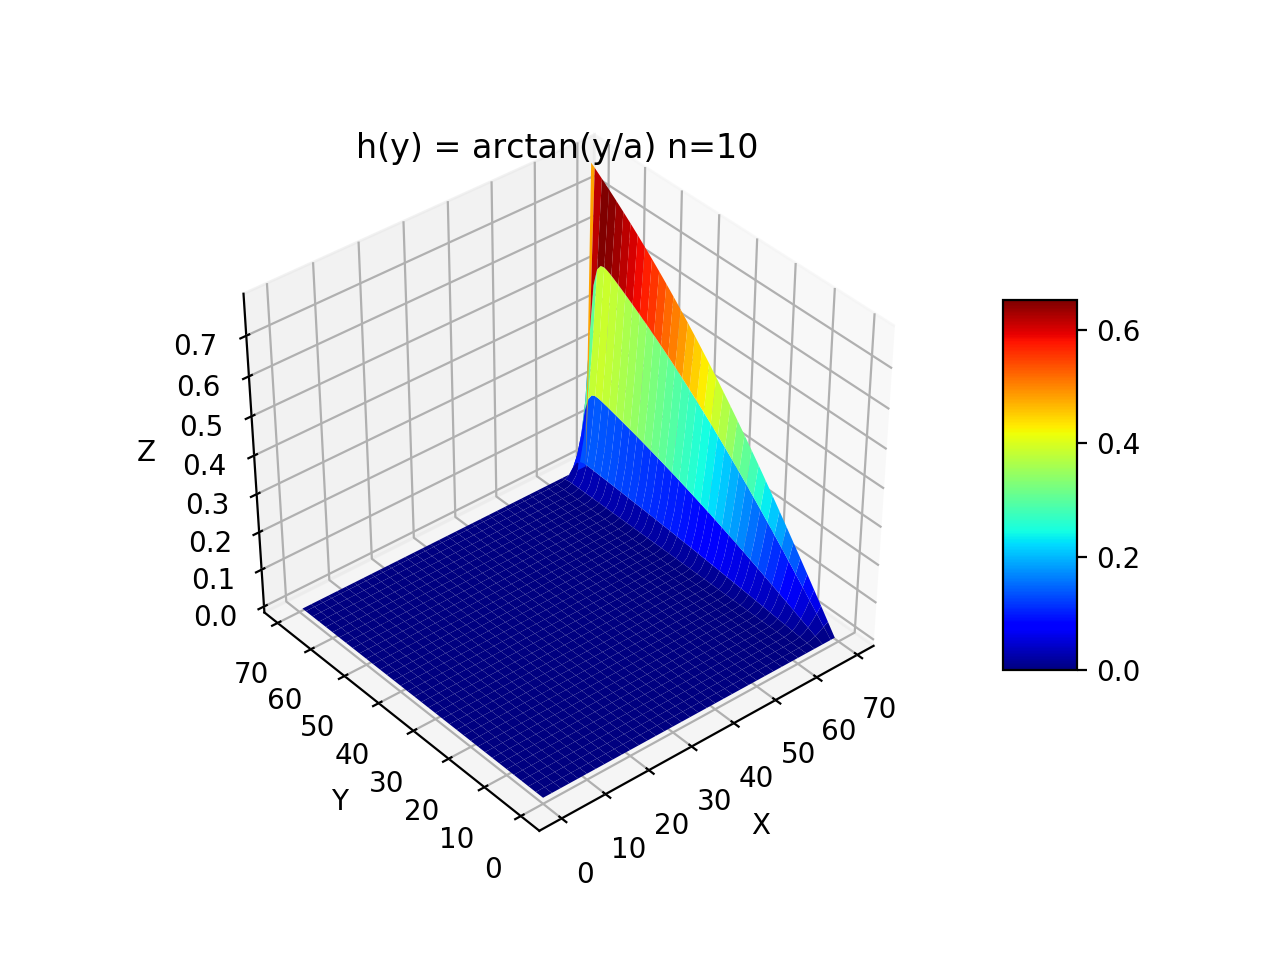
\includegraphics[width=1.5in]{images/arctan-n10}
  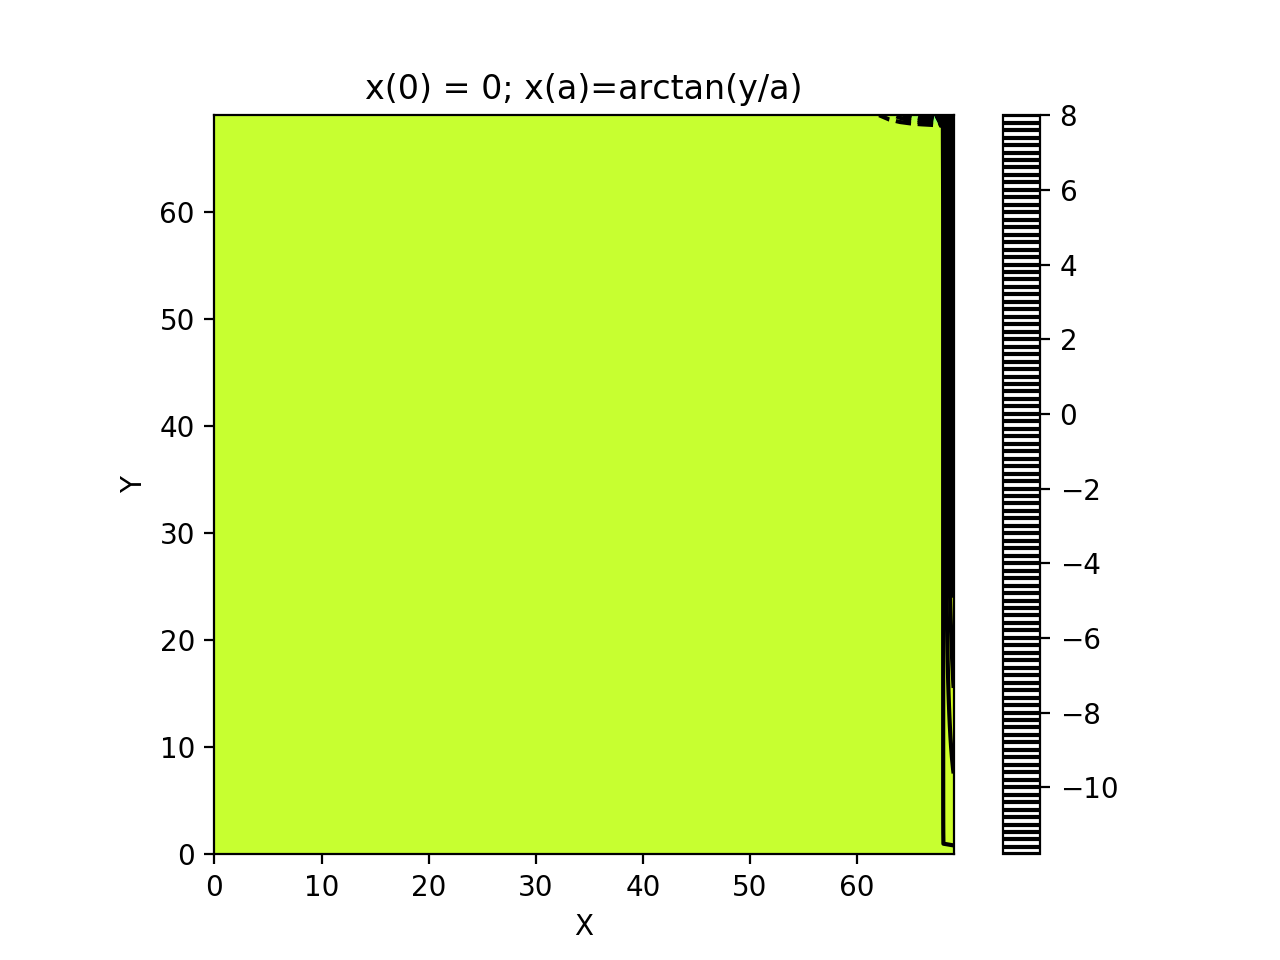
\includegraphics[width=1.5in]{images/arctan-density}
  \caption{\(h(y) = tan^{-1}(y/a)\) con iteraciones \(n = 0, 2, 5 \text{ y } 10\)}
  \label{arctan-iterations}
\end{figure}

Para este inciso se requiere resolver una forma alternativa en la que se elimina
el plano \(x=0\), para esta configuración se asumirá que el campo naturalmente tiene un
potencial de 0.1v para poder apreciar el efecto de los planos conectados a tierra.
\\\\
Como ya se incluye detalles de la solución anterior, solo mostraremos los graficos de \(n=20\).

\begin{figure}
  \centering
  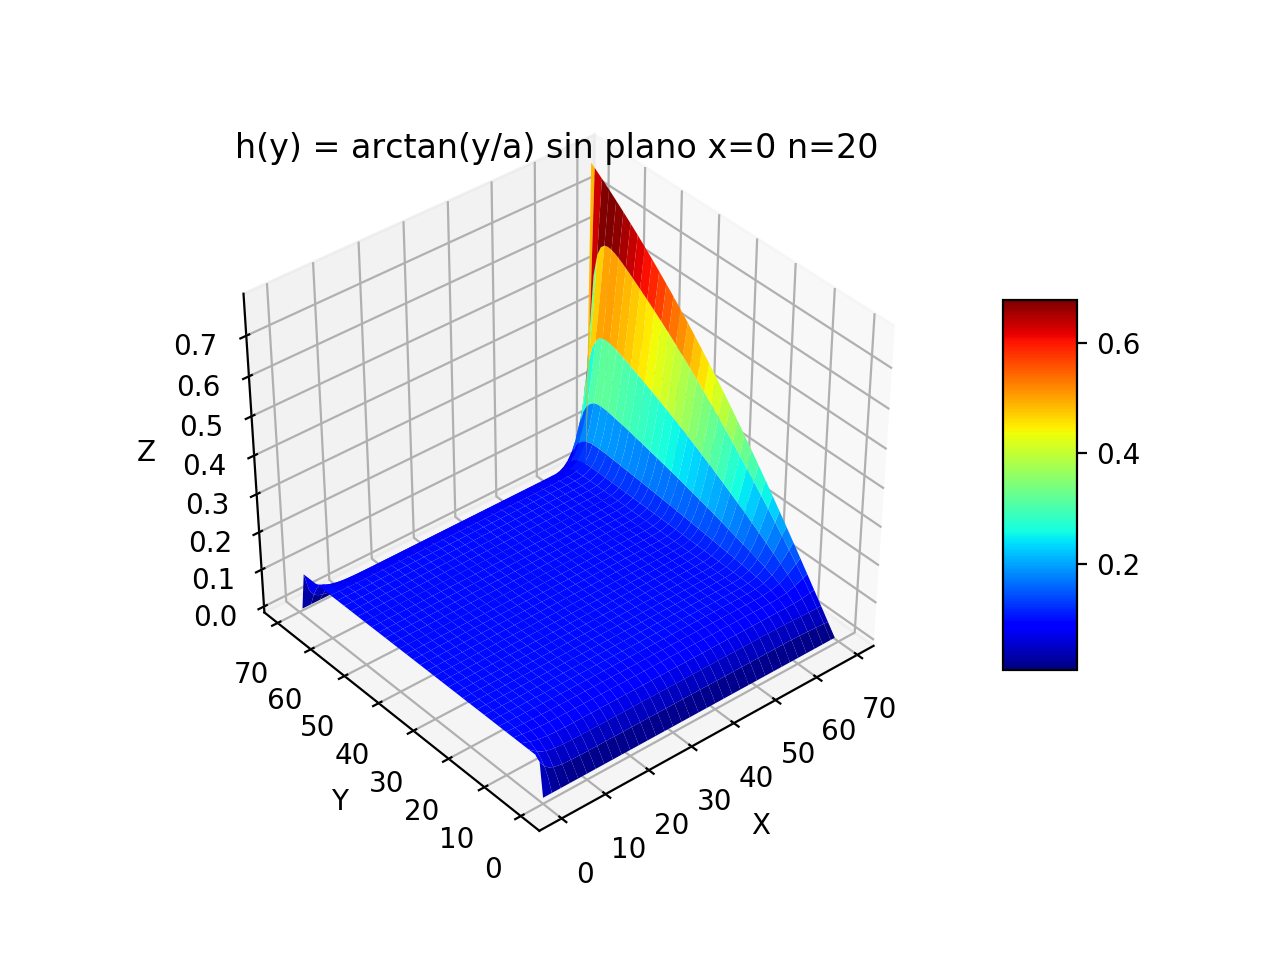
\includegraphics[width=2.8in]{images/arctan-alt-n20}
  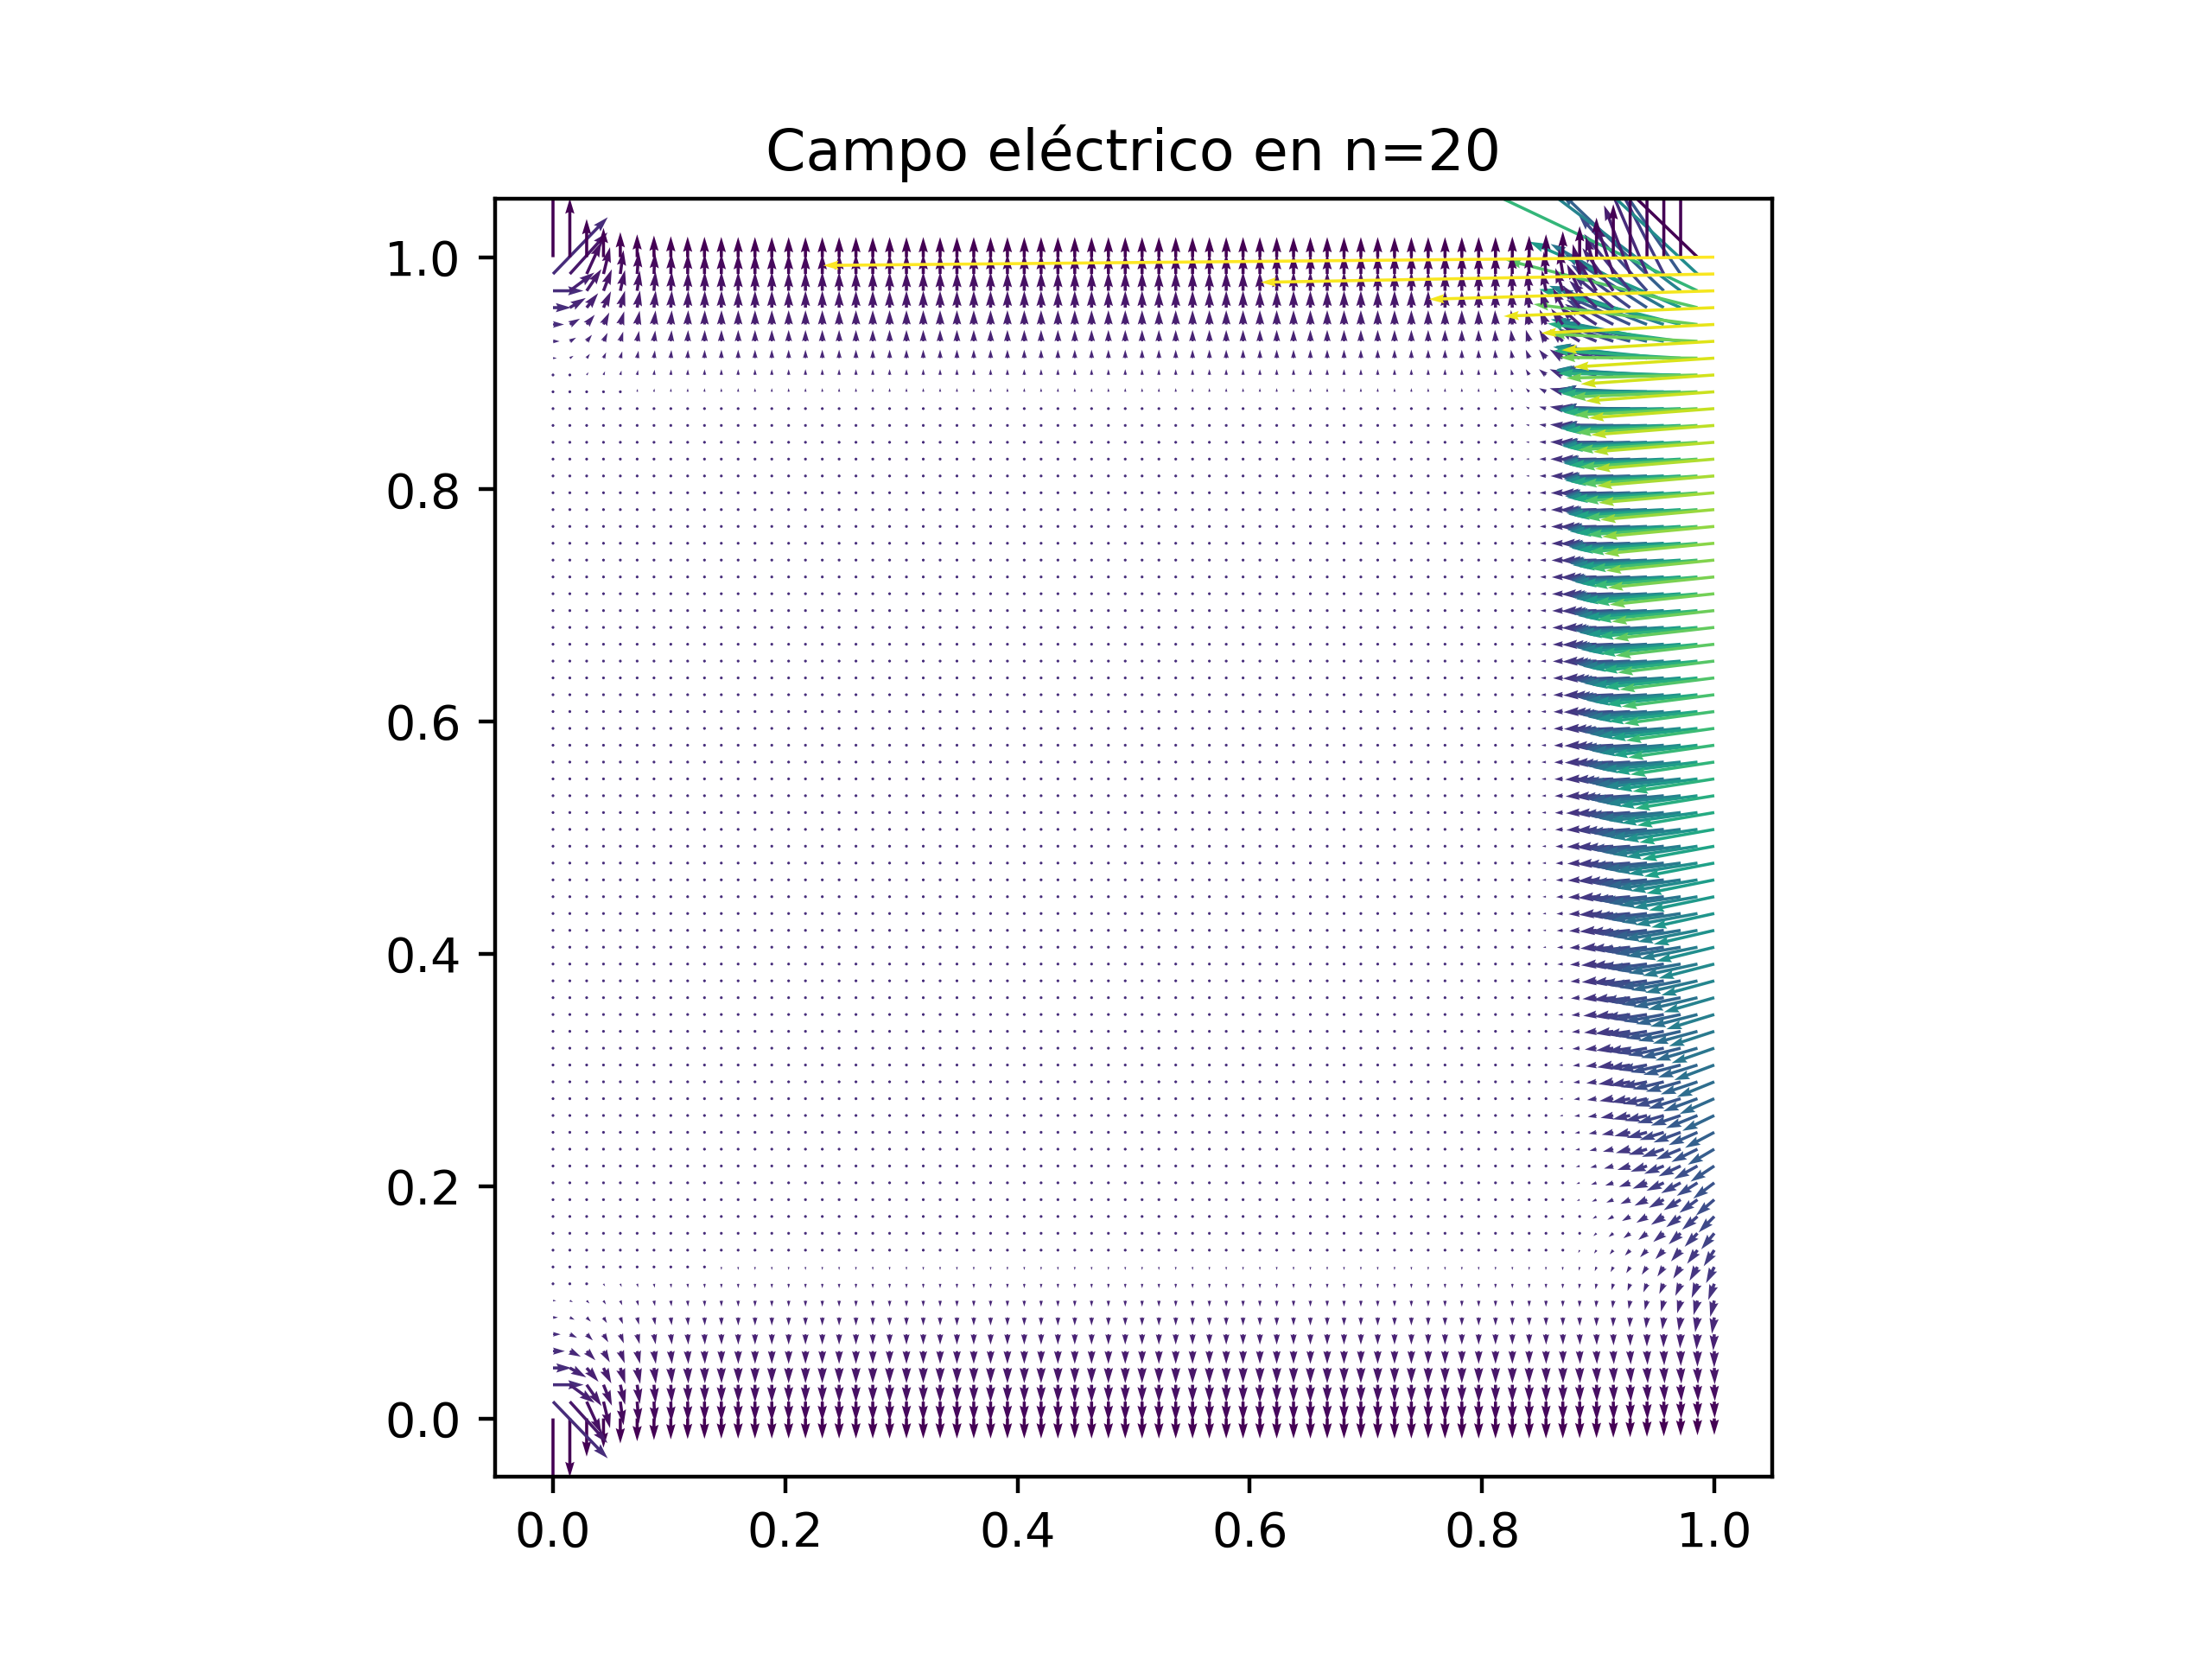
\includegraphics[width=2.8in]{images/arctan-alt-field}
  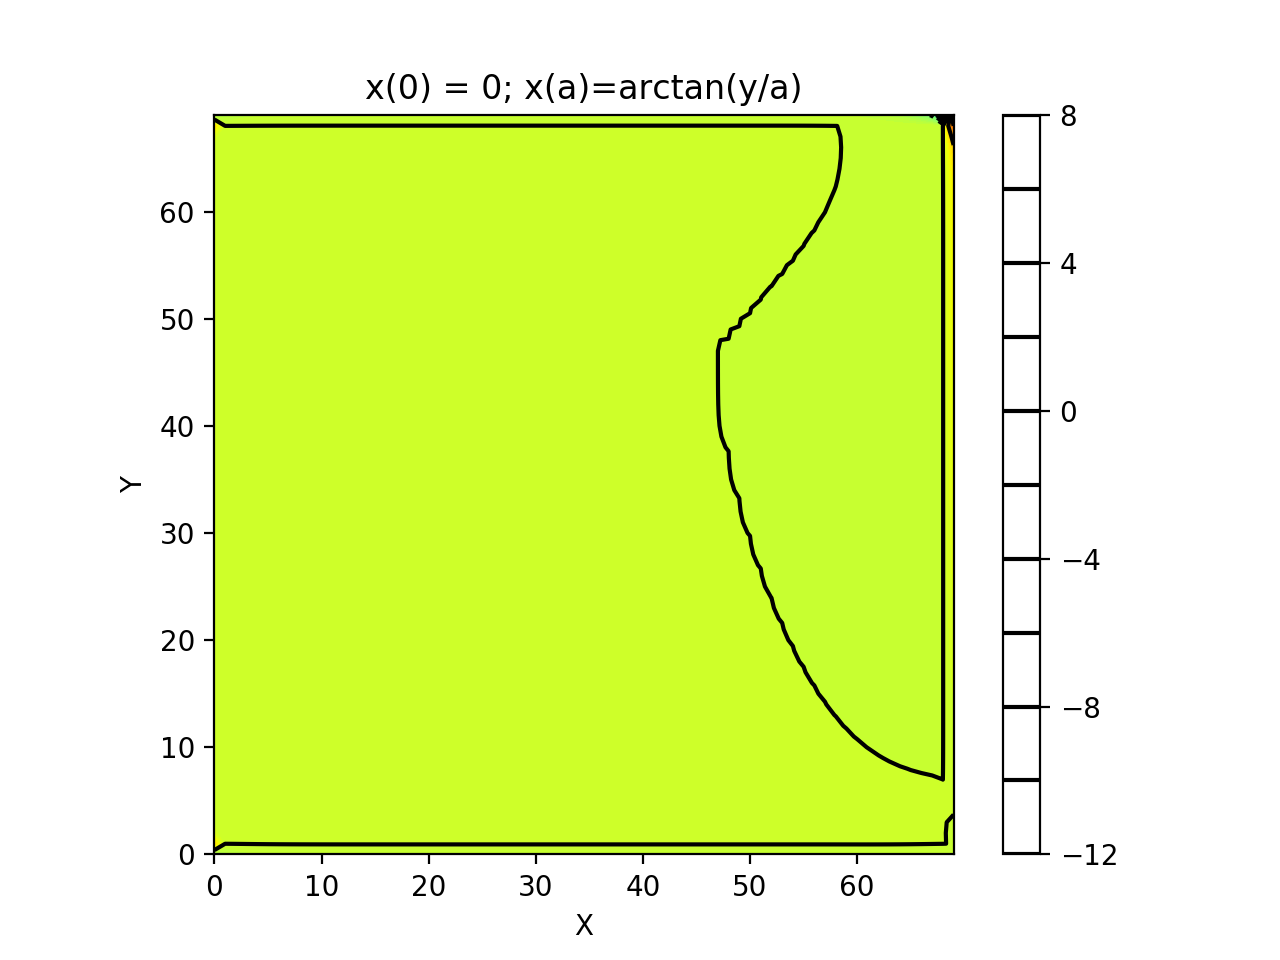
\includegraphics[width=1.5in]{images/arctan-alt-density}
  \caption{Potencial, campo eléctrico para \(h(y) = tan^{-1}(y/a) sin x=0\)}
  \label{arctan-n20}
\end{figure}


\pagebreak

\subsubsection{Cambio de condiciones}

Si el plano \(x=0\) se corre a \(x=-b\), y se tiene
\\
\(g(y)=h(y)=2y^3+5\) 
\\\\
Para este inciso se necesitan dos condiciones de frontera distintas de cero y valores en el plano negativo.
Gracias a que función de condicion de frontera es independiente de \(x\) simplemente duplicaremos el tamaño del
espacio en ese eje, es decir las condiciones iniciales se presentarán en \(x=0, x=2b\).

\subsubsection{Solución analítica}

\begin{align*}
  &\text{Tomamos la ecuación original y aplicamos condiciones}\\
  &V(\pm x,y) = 2y^3 + 5 \text{ Simetría en X, permite cambiar} \\
  A &= B, e^{kx} + e^{-kx} = 2A*2cosh(kt)\\
  V(x,y) &= cosh(kt)(C sin(ky) + D cos(ky)),\\
  V(x,0) &= cosh(kt)(C sin(ky) + \cancelto{0}{D} cos(ky)) = 0\\
  V(x,a) &= 0, k = \frac{n*pi}{a}\\
  V(b,y) &= \sum_{n=1}^{\infty} C_n cosh(\frac{n\pi x}{a}) sin(\frac{n\pi x}{a}) = 2y^3 + 5\\
  \\
  &\text{Truco de Fourier}\\
  C_n& cosh(\frac{n\pi b}{a}) = \frac{4V_o}{n\pi}, \text{si n es impar}\\
  V(b,y) &= \frac{4V_o}{\pi}(2y^3 + 5) \sum_{n=1}^{\infty} \frac{1}{n} * \frac{cosh(\frac{n\pi x}{a})}{cosh(\frac{n\pi b}{a})} sin(\frac{n\pi y}{a})
\end{align*}

\subsubsection{Solución numérica}

En el código las configuramos de esta forma
\begin{lstlisting}
  T[:,-1] = 2*y**3+5
  T[:,0] = 2*y**3+5
\end{lstlisting}

\begin{figure}
  \centering
  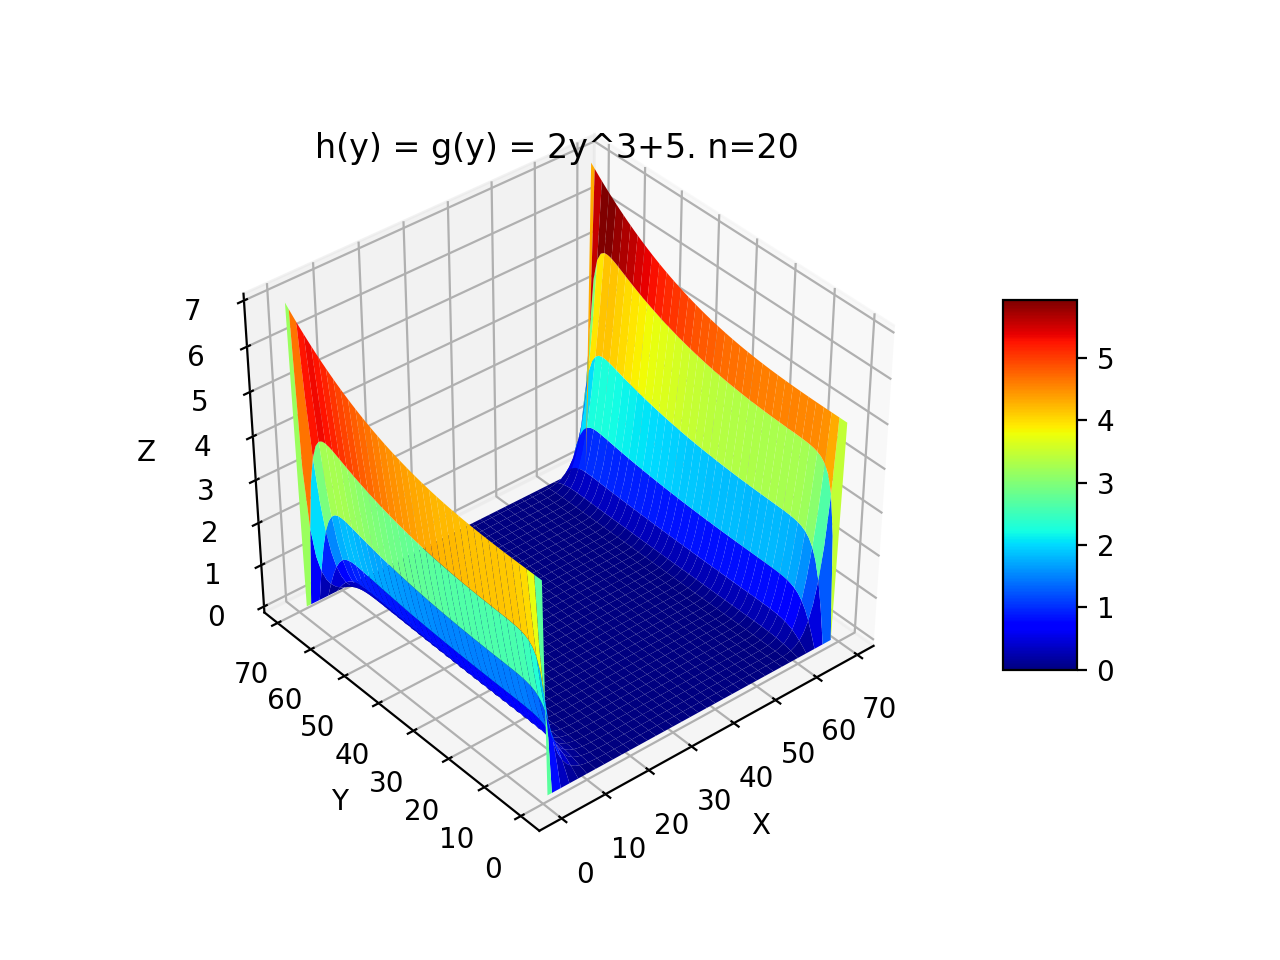
\includegraphics[width=2.8in]{images/2y3-n20}
  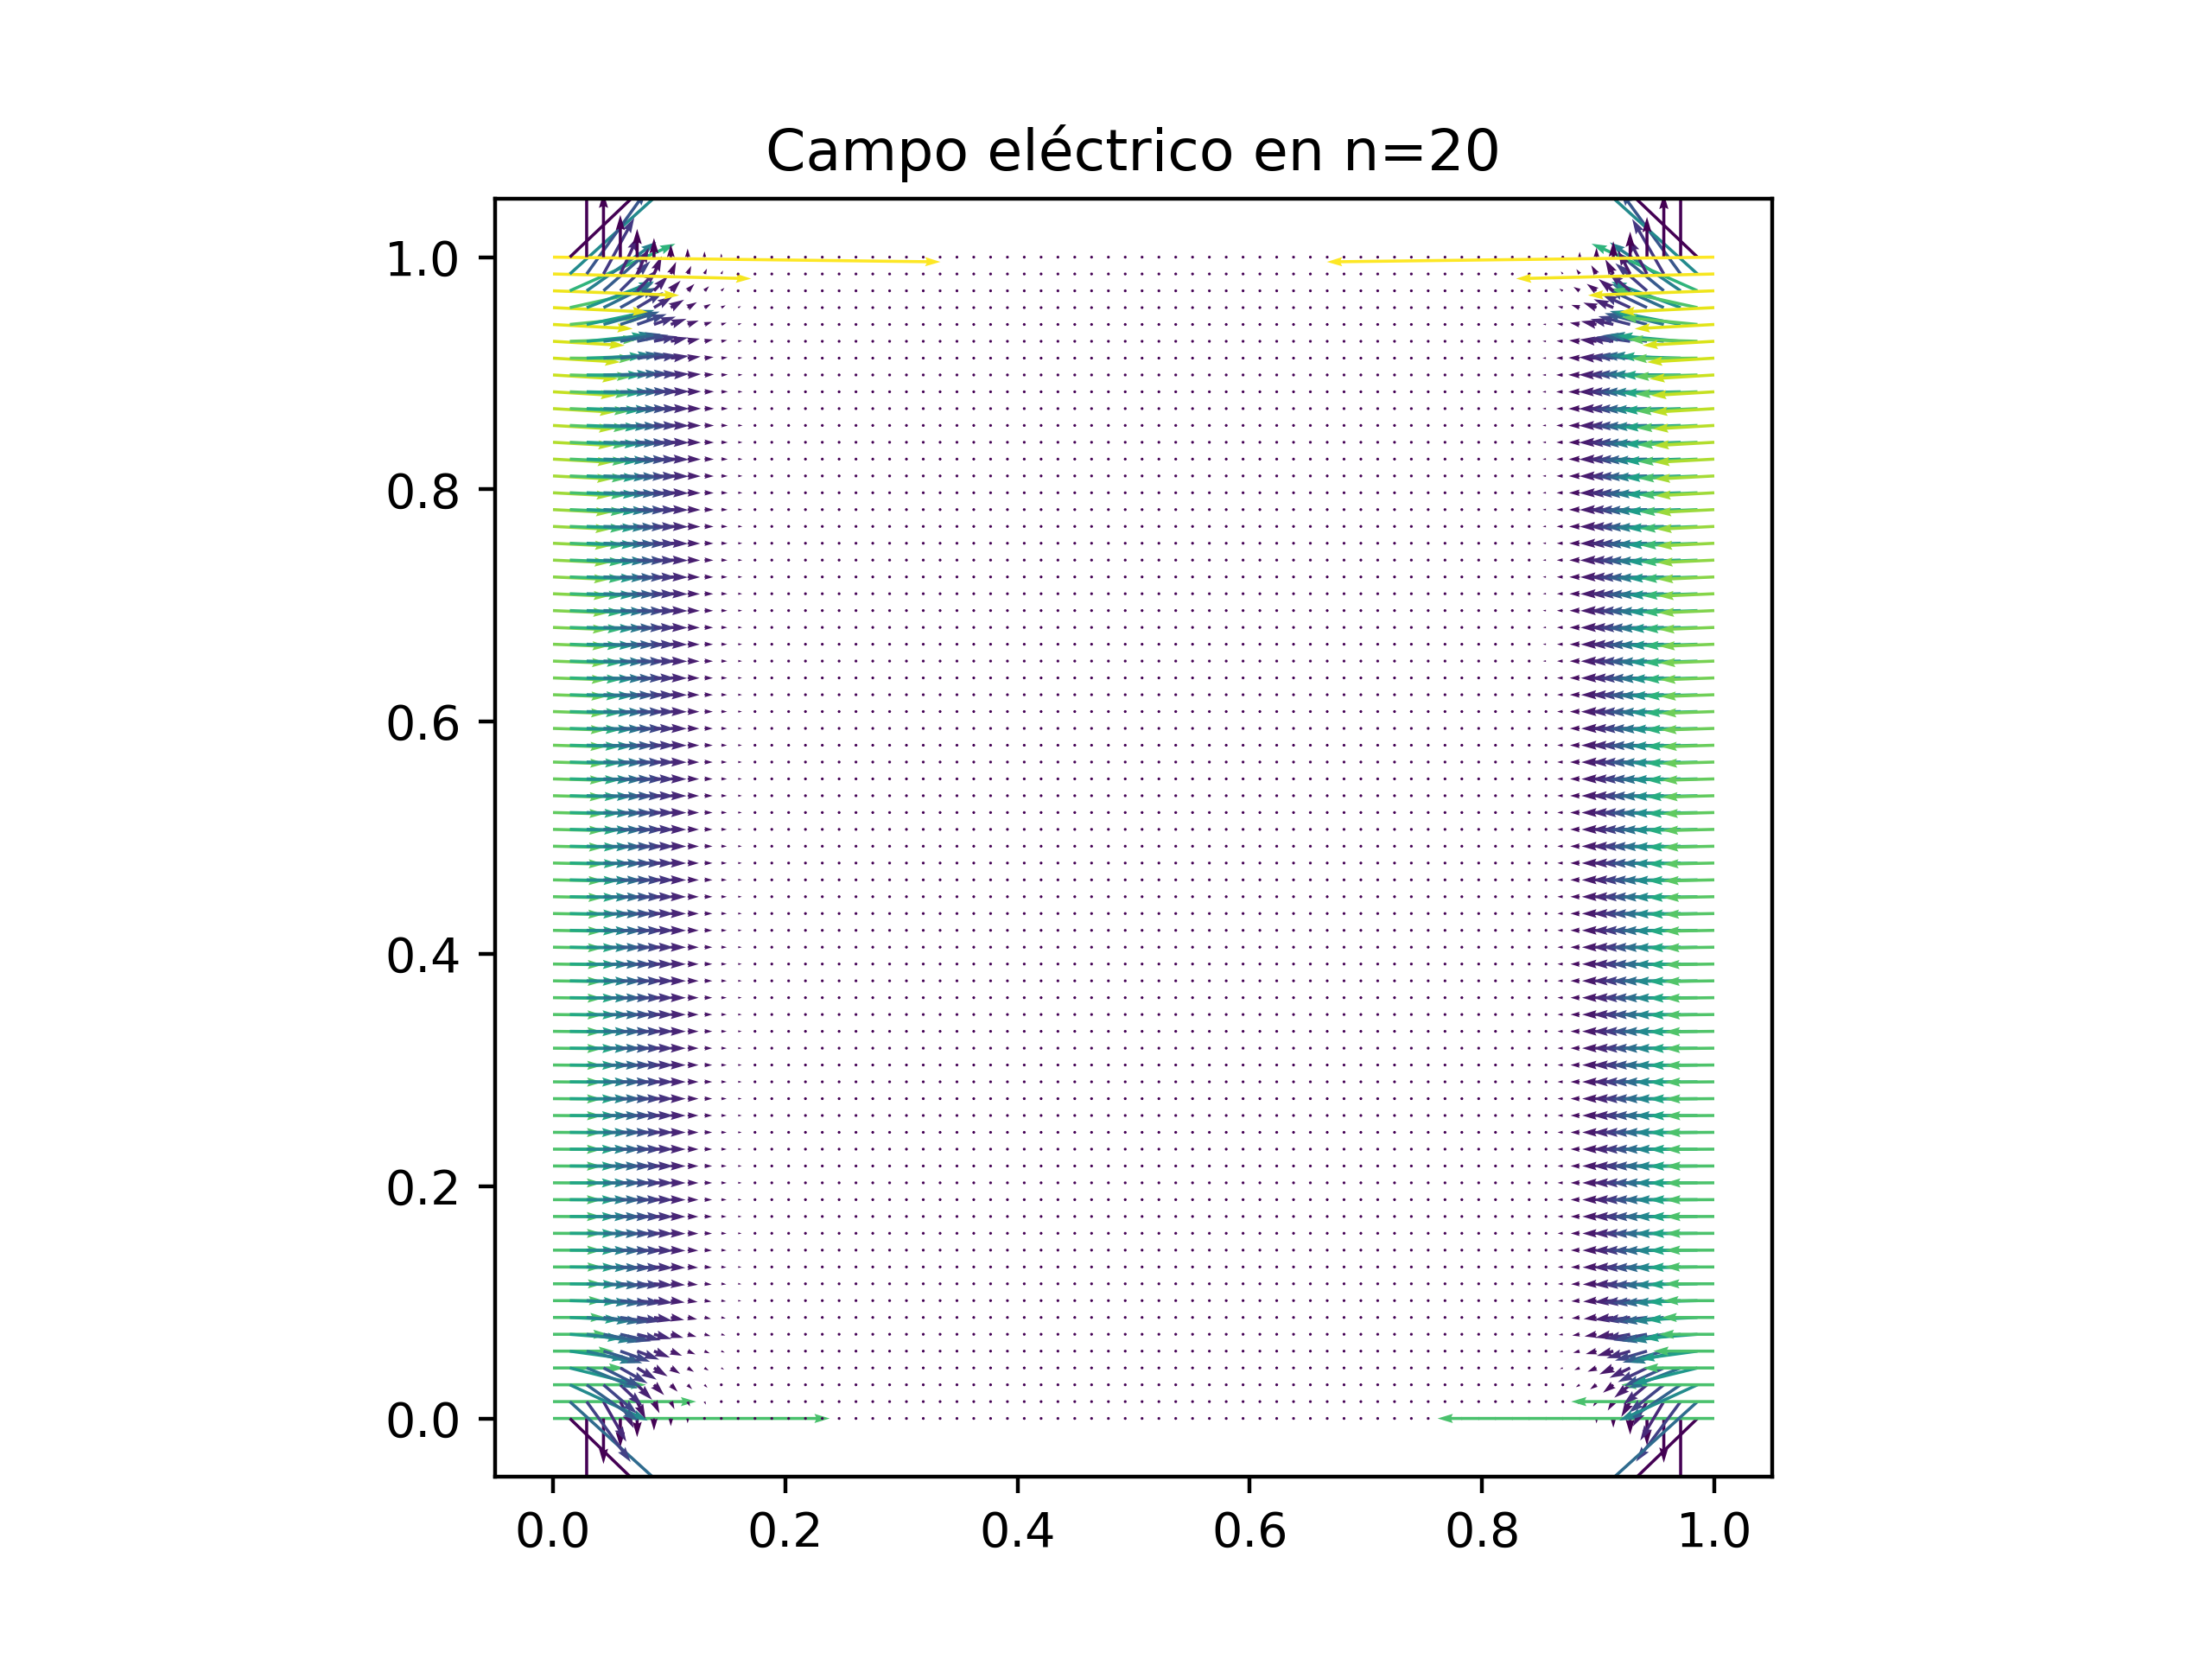
\includegraphics[width=2.8in]{images/2y3-field}
  \caption{Potencial y campo eléctrico para \(h(y) = g(y) = 2y^3+5\)}
  \label{2y3-n20}
\end{figure}

\begin{figure}
  \centering
  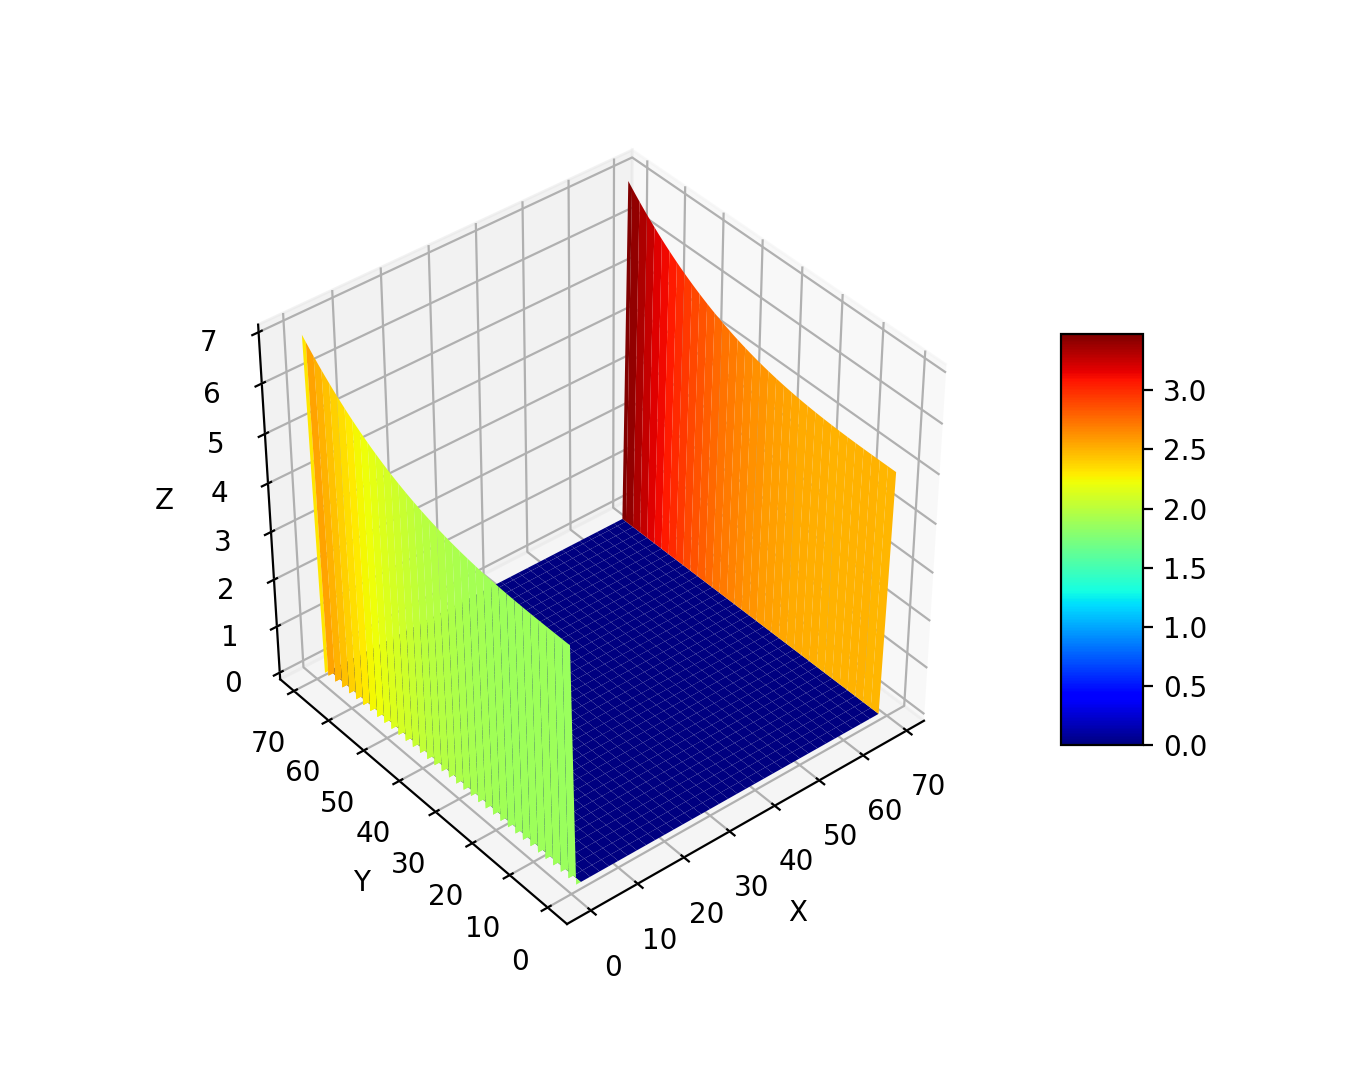
\includegraphics[width=1.5in]{images/2y3-n0}
  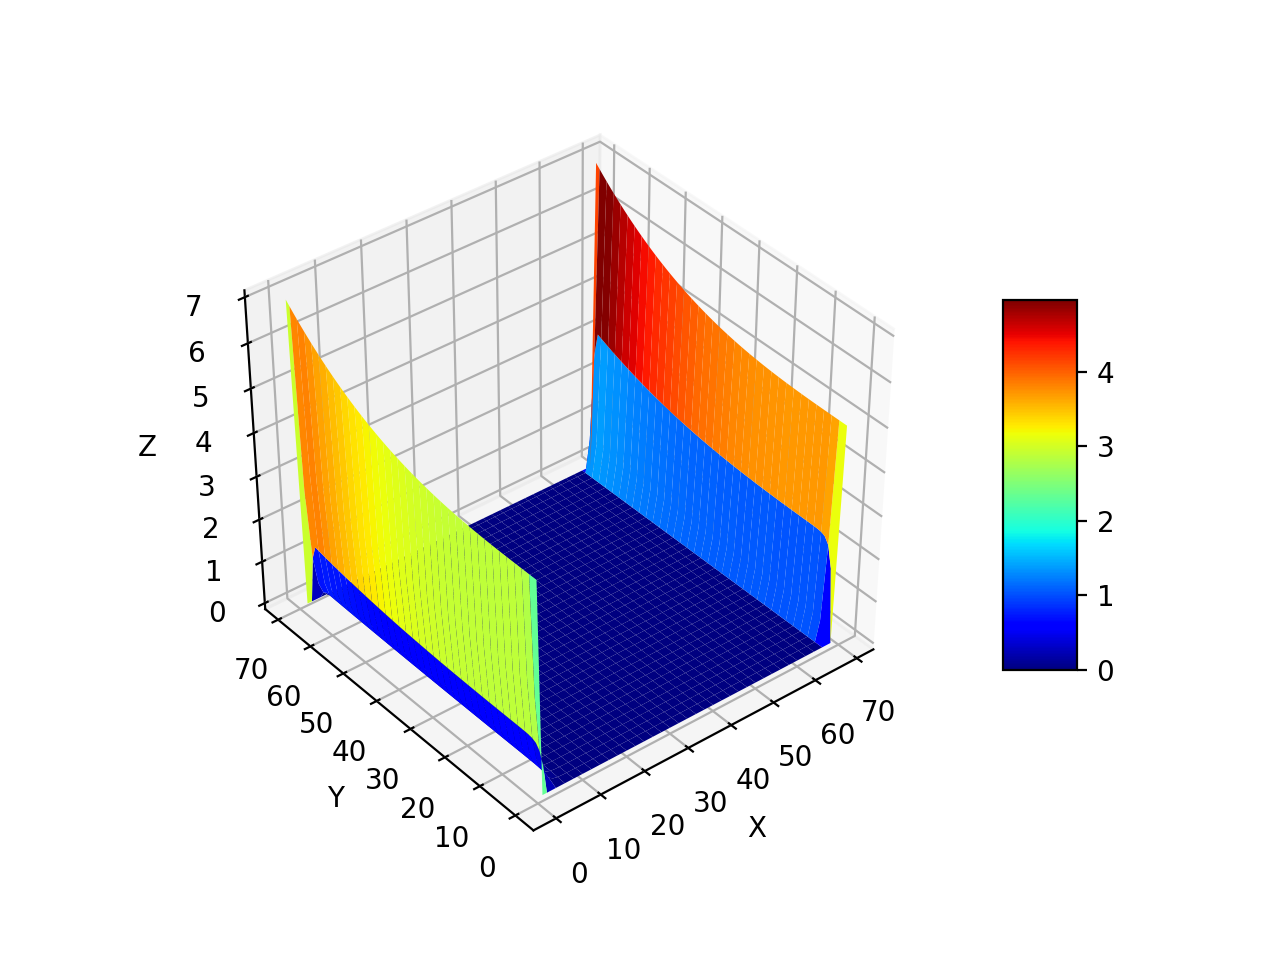
\includegraphics[width=1.5in]{images/2y3-n2}
  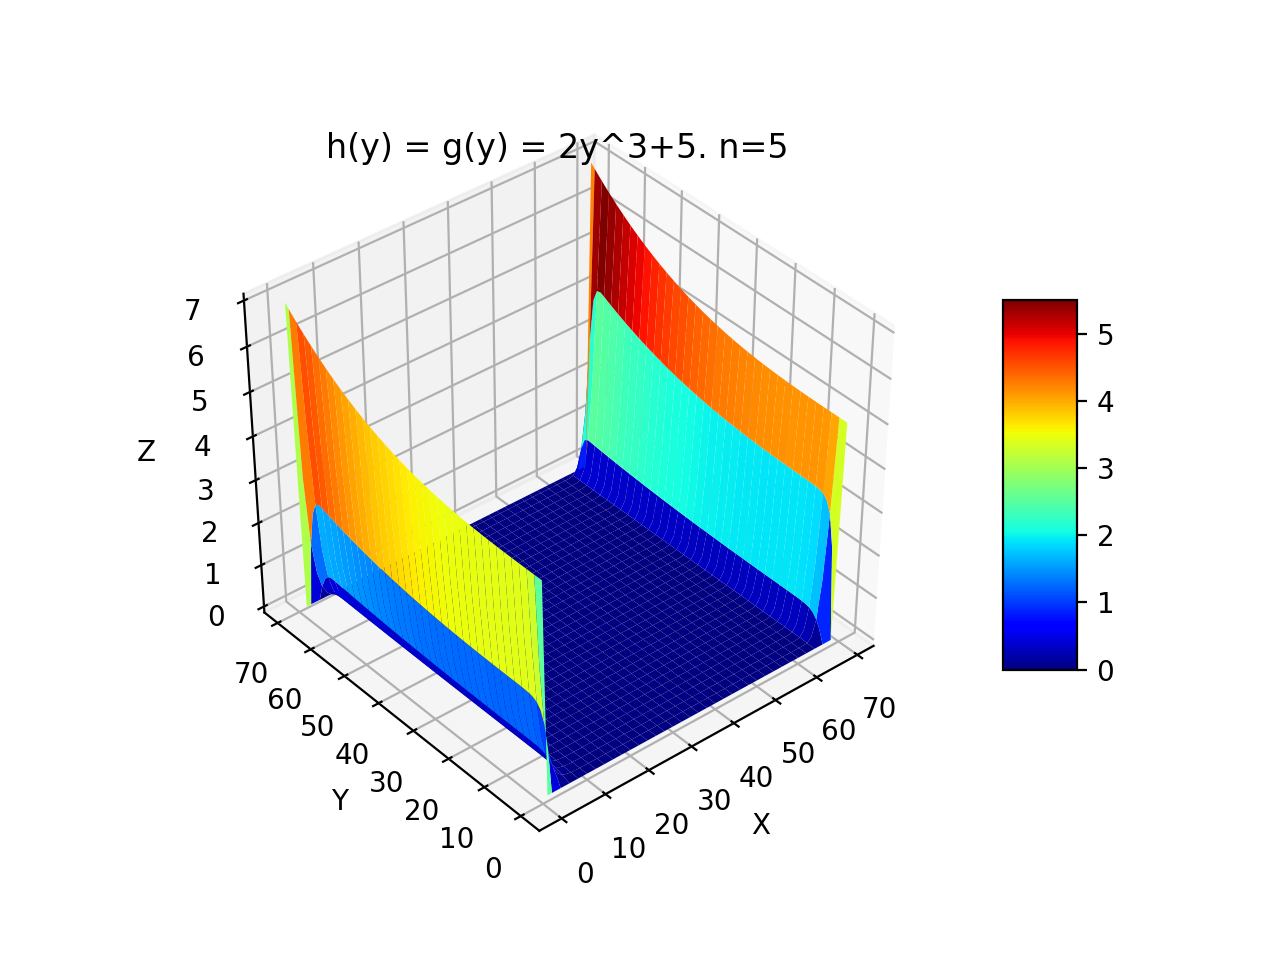
\includegraphics[width=1.5in]{images/2y3-n5}
  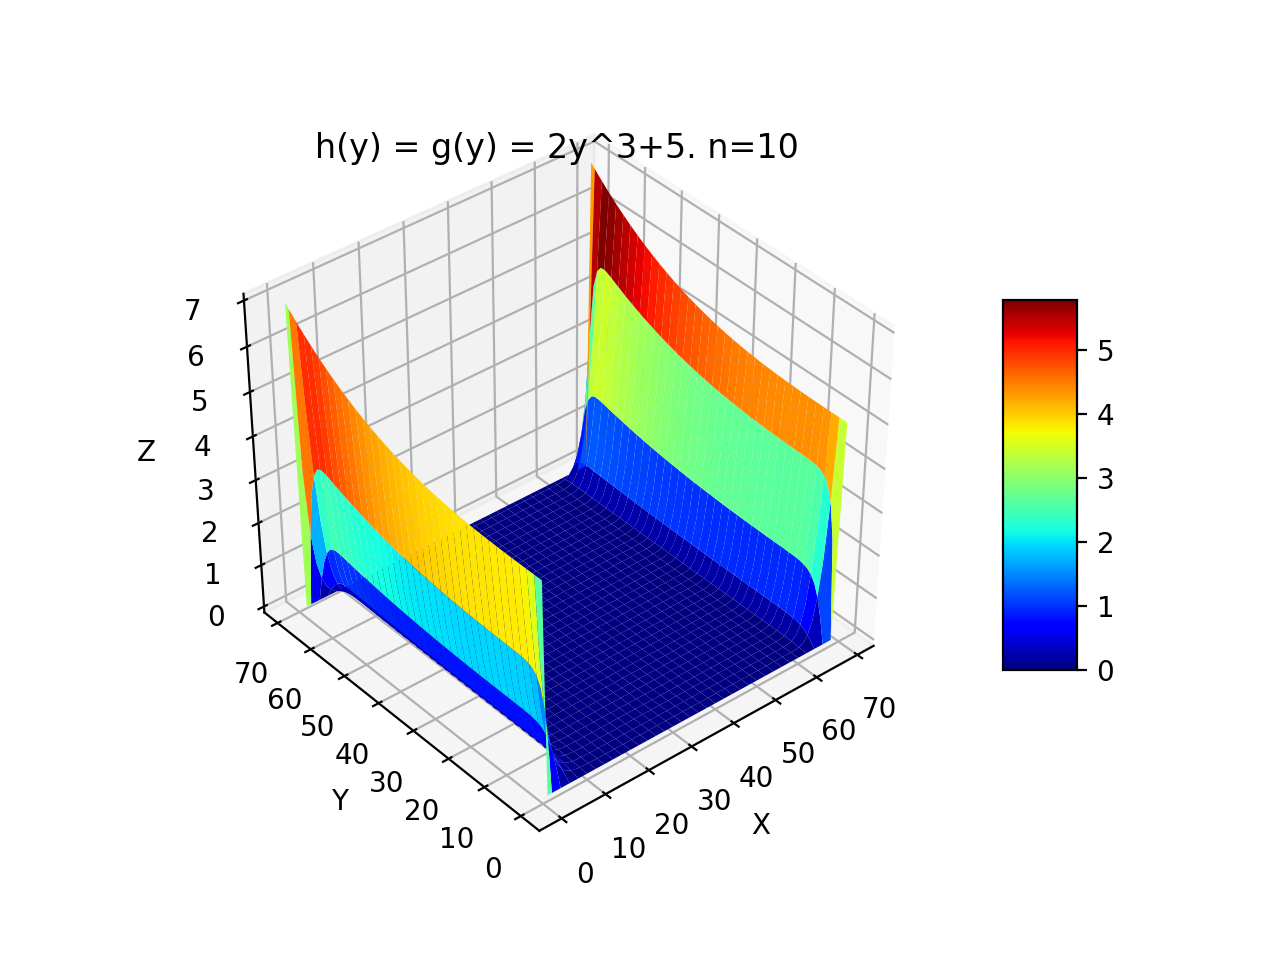
\includegraphics[width=1.5in]{images/2y3-n10}
  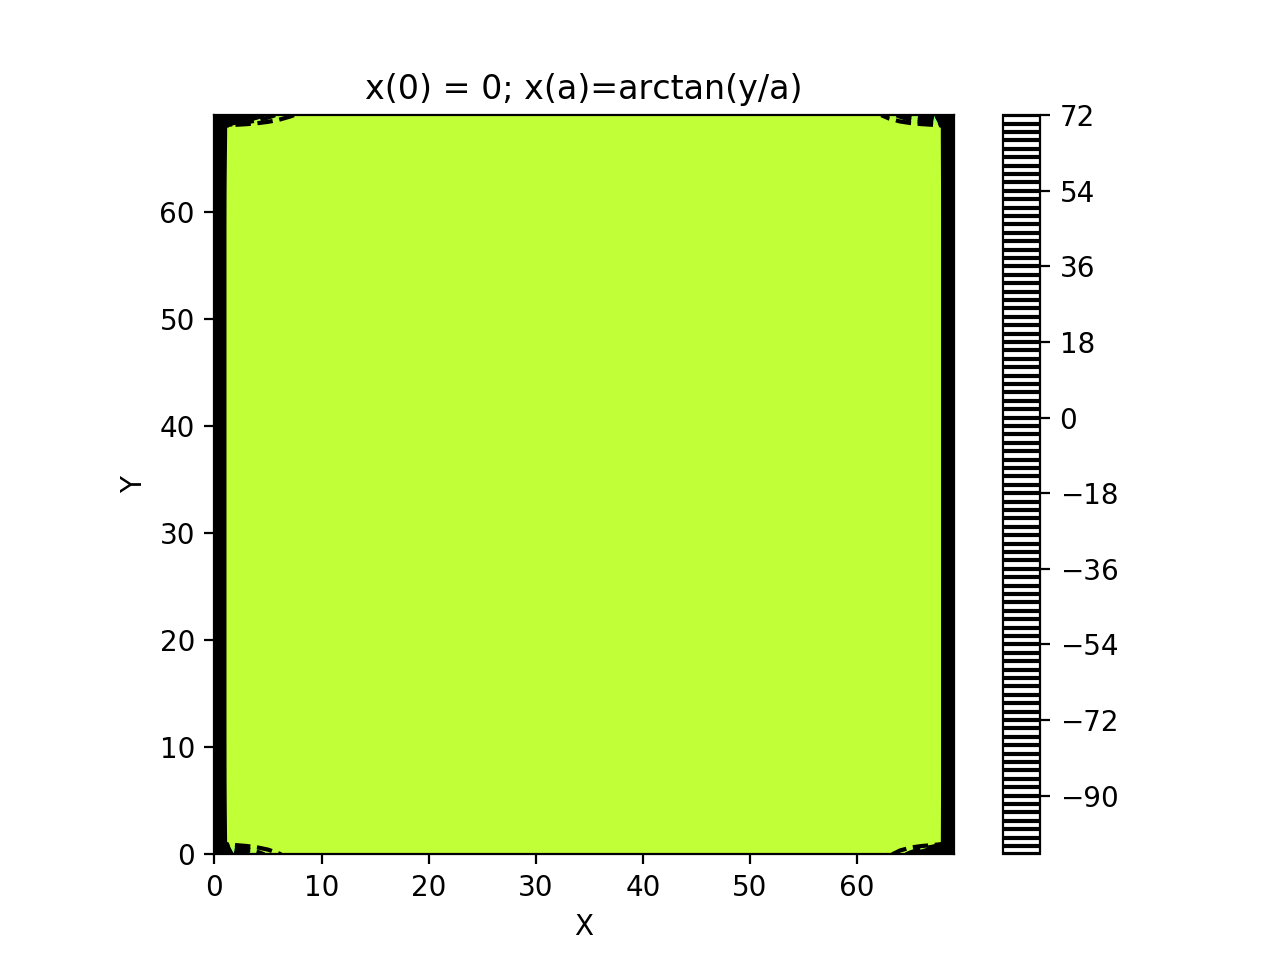
\includegraphics[width=1.5in]{images/2y3-density}
  \caption{\(h(y) = g(y) = 2y^3+5\) con iteraciones \(n = 0, 2, 5 \text{ y } 10\)}
  \label{2y3-iterations}
\end{figure}

Así como el ejercicio anterior, presentamos el mapa de calor y el campo eléctrico de la iteración \(n=20\) en la figura \ref{2y3-n20} seguido de 
las iteraciones menores, densidad y condiciones iniciales (figura \ref{2y3-iterations}).


/subsubsection{Problema de Laplace en 3D}

Una tubería se extiende a lo largo del eje z
y posee paredes en \(x = y = z=0,x=a y=b\). La placa en \(z=0\) se encuentra a potencial
\(f(x,y) = xy^2\), y las demás están aterrizadas.
Elija valores de a y b de tal manera que las gráficas puedan apreciarse correctamente.
Realice las gráficas para \(n= 2, 5, 10, 20\)

Para poder graficar correctamente este ejercicio, utilizaremos la misma función de antes para
generar mapas de calor en 3D, pero en este caso agregaremos distintos nuevos para valores de z.

Utilizando matplotlib, es facil agregar planos utilizando:
\subsubsection{Solución analítica}

Este es claramente un problema en 3D, y para eso actualizaremos la ecuación
\begin{align*}
  X(x) &= Ae^{sqrt(k^2+l^2)x} + Be^{sqrt(k^2+l^2)x}\\
  Y(y) &= C sin(ky) + D cos(ky)\\
  Z(z) &= E sin (lz) + F cos(lz)\\
  \\
  &\text{Todos los coeficientes de X son cero,}\\
  &D = 0\\
  &k = \frac{\pi n}{b}\\
  &\text{Simplificando como antes obtenemos}\\
  V &= xy^2 \sum_{n=1}^{\infty} \sum_{m=1}^{\infty} C_nm sin(\frac{n \pi}{a})sin(\frac{m x\pi}{b})\\
  C &= \frac{4}{ab} \int_0^a \int_0^b xy^2 sin(\frac{n \pi}{a})sin(\frac{m x\pi}{b}) dydx
\end{align*}


\subsubsection{Solución numérica}
\begin{lstlisting}
  # agregamos alpha para ver los planos
  ax.plot_surface(x,y,field[z]+z, alpha=0.3)
\end{lstlisting}

El otro cambio que debemos hacer es adaptar la función de relajación para funcionar en un campo 3D.
Basta con agregar:
\begin{lstlisting}
  # Agregamos otra dimension
  field[i, j, k] = 1/6 * \
  (field[i+1][j][k] ...  \
  field[i][j][k+1] + field[i][j][k-1])
\end{lstlisting}

Finalmente iteramos la nueva función con los arreglos y obtenemos un excelente resultado mostrado en 
figura \ref{xy2-n20}, como siempre, las iteraciones menores a menor detalle en \ref{xy2-iterations}

\begin{figure}
  \centering
  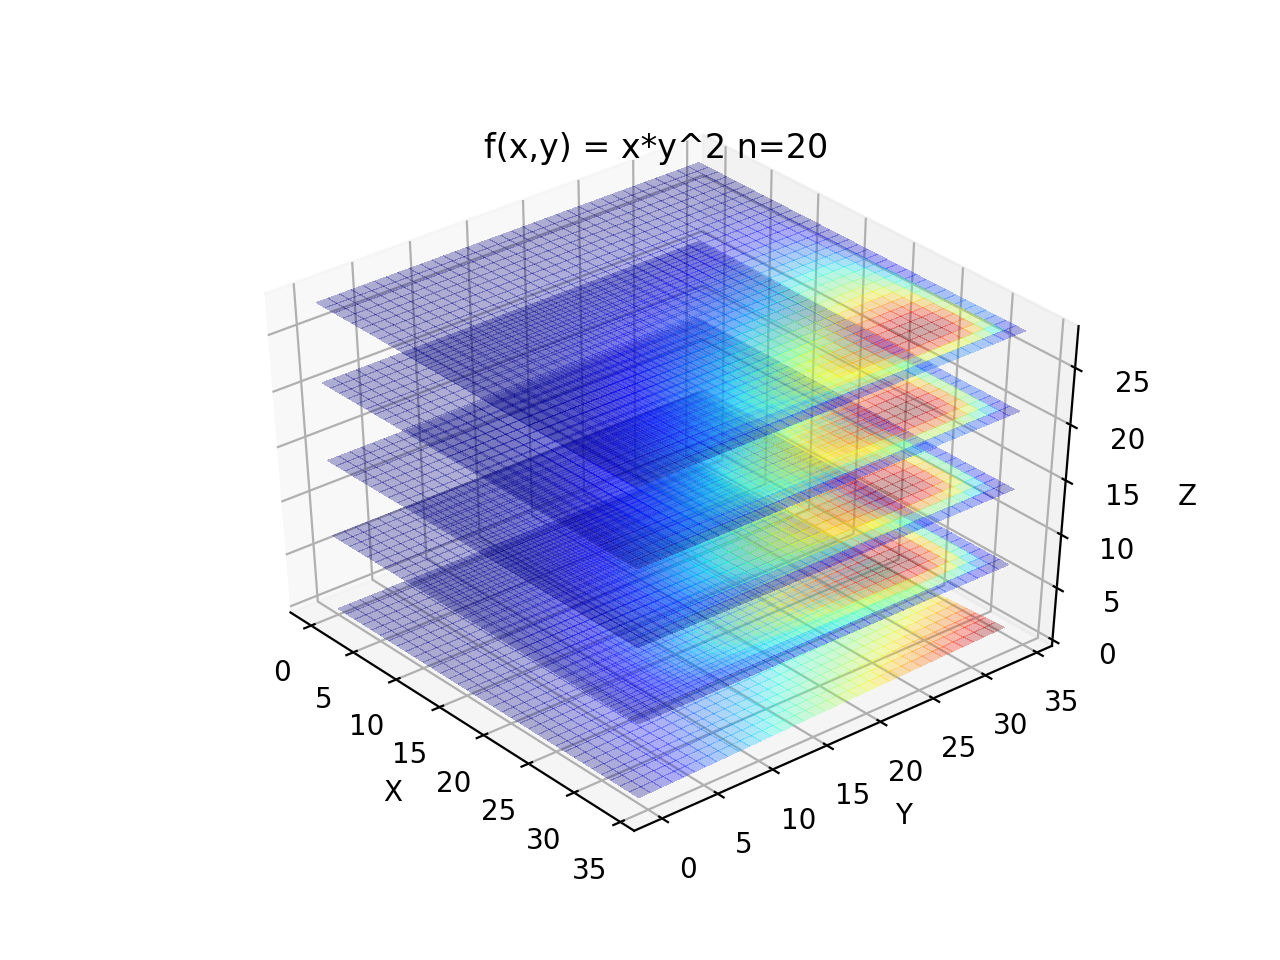
\includegraphics[width=2.8in]{images/xy2-n20}
  \caption{Potencial y campo eléctrico para \(f(x,y) = xy^2\)}
  \label{xy2-n20}
\end{figure}

\begin{figure}
  \centering
  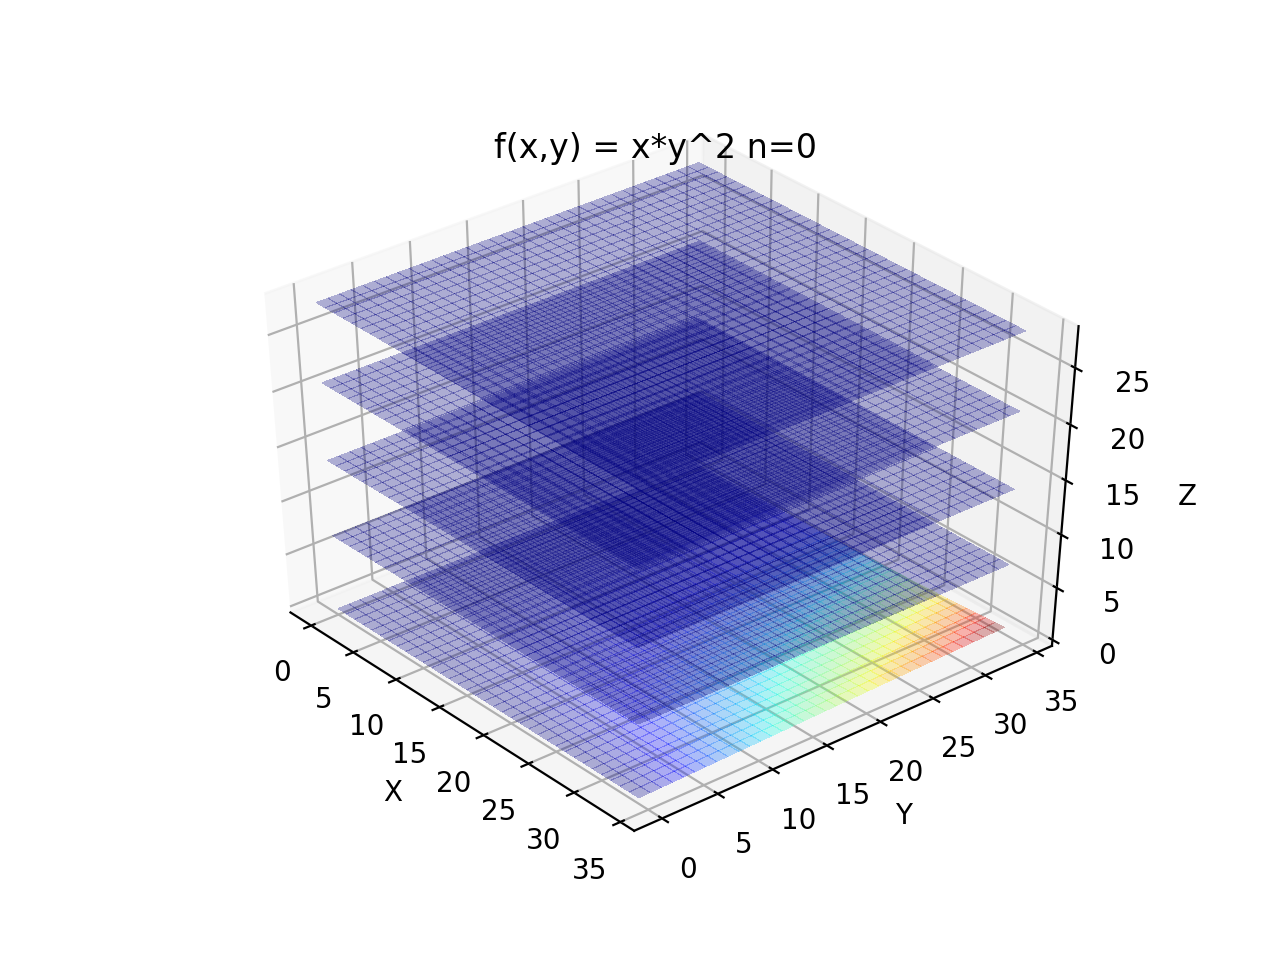
\includegraphics[width=1.5in]{images/xy2-n0}
  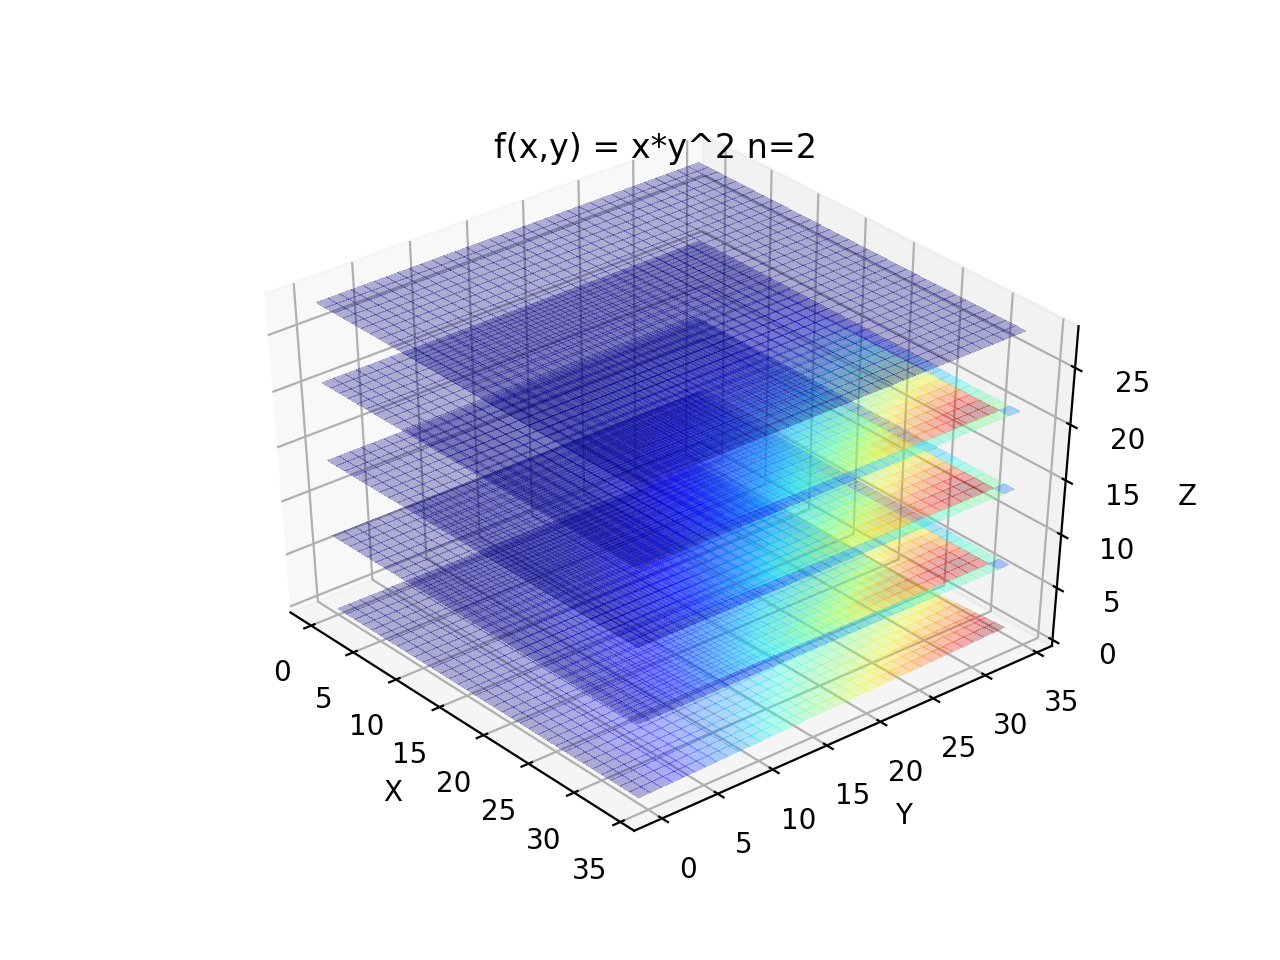
\includegraphics[width=1.5in]{images/xy2-n2}
  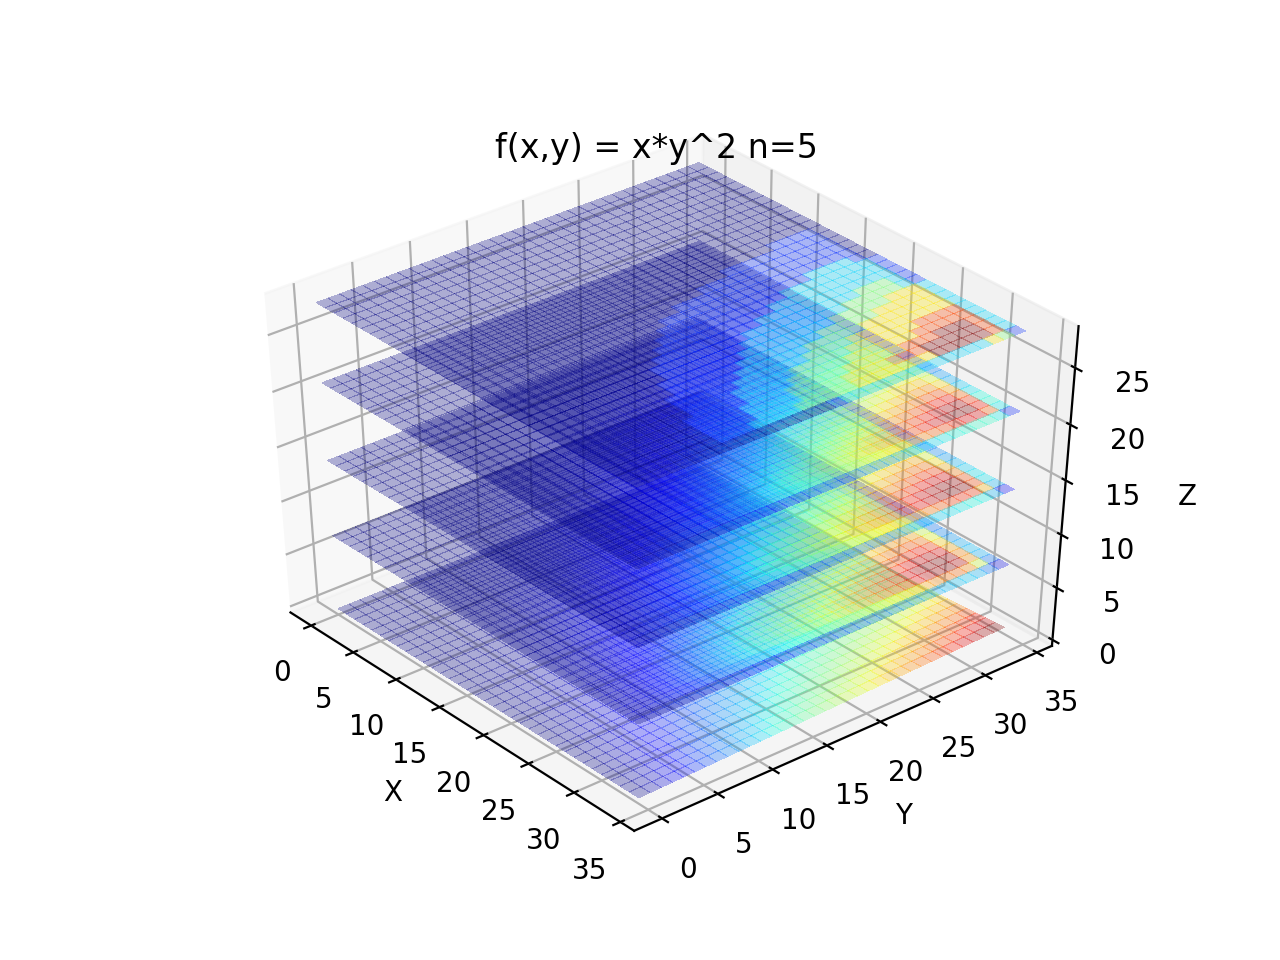
\includegraphics[width=1.5in]{images/xy2-n5}
  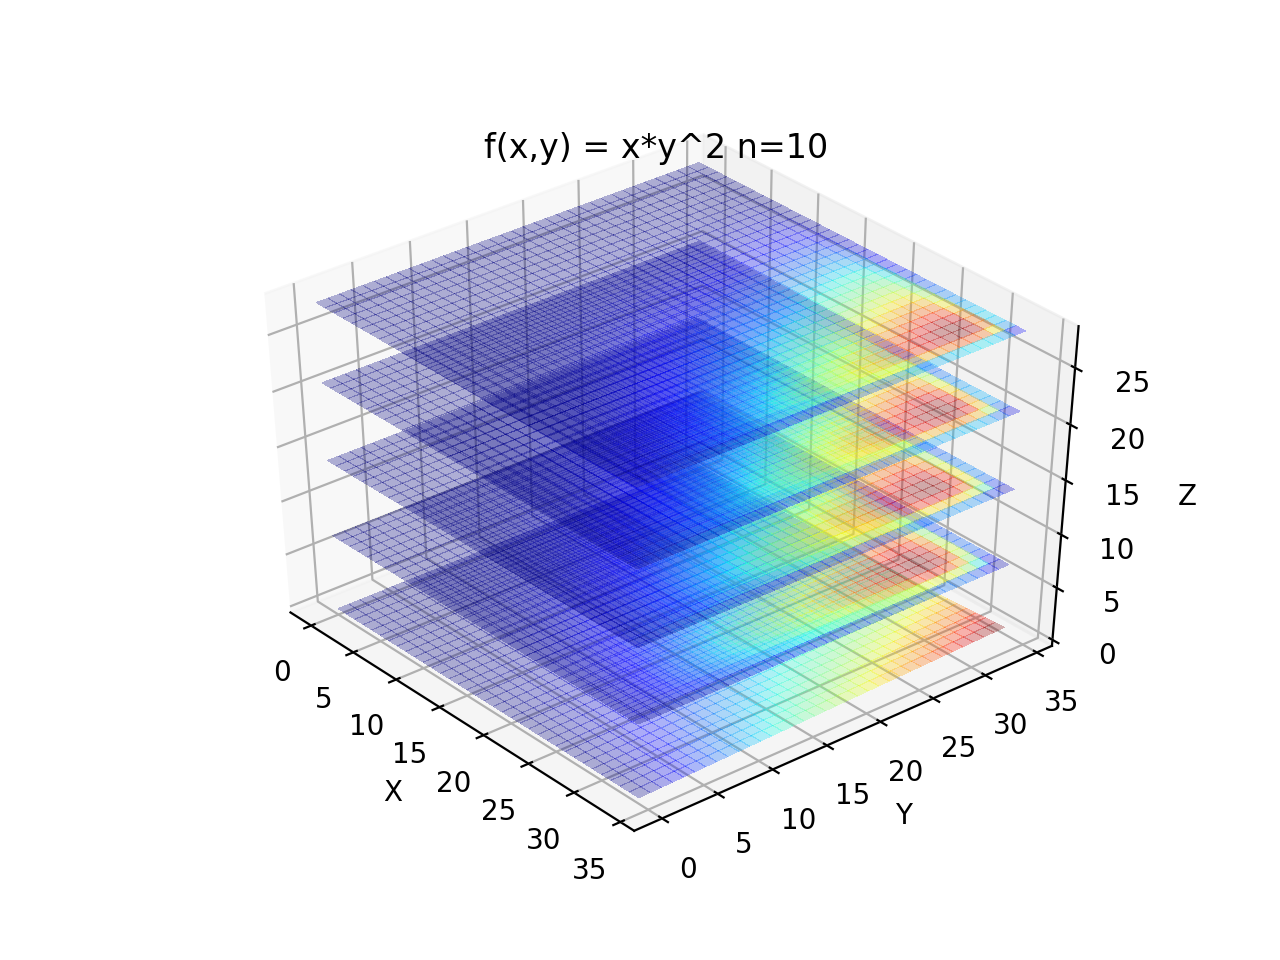
\includegraphics[width=1.5in]{images/xy2-n10}
  \caption{\(h(y) = g(y) = 2y^3+5\) con iteraciones \(n = 0, 2, 5 \text{ y } 10\)}
  \label{xy2-iterations}
\end{figure}


\subsection{Ecuación de Laplace en coordenadas esféricas}

Una esfera de radio R cuya densidad de carga superficial está dada por\\

\begin{align*}
  \sigma(\theta) &= -3/2cos(3\theta) \\
  \Delta f&={\frac {1}{r}}{\frac {\partial ^{2}}{\partial r^{2}}}(rf)+{\frac {1}{r^{2}\sin \theta }}{\frac {\partial }{\partial \theta }}\left(\sin \theta {\frac {\partial f}{\partial \theta }}\right)+{\frac {1}{r^{2}\sin ^{2}\theta }}{\frac {\partial ^{2}f}{\partial \varphi ^{2}}}\\
\end{align*}

Solución 
\begin{align*}
  &\text{Condiciones de frontera}\\
  \phi(r=0, \theta) &= \exists \quad \phi(r=R, \theta) = -3/2cos(3\theta)\\
  r &= R: \theta_{dentro} = \theta{fuera} \quad V \to 0, \phi \to \infty 
\end{align*}

\section{Conclusión}

A pesar de que se requirere matemática y conocimentos relativamente avanzados,
la Ecuación de Laplace se comporta intuitivamente y es facil de predecir.

\appendices
\section{Formas alternativas de calcular campos potenciales}

\subsubsection{Relajación por Jacobi}

La forma más común de calcular numericamente la ecuación de Laplace
consta en escoger un "5 point stencil" o lienzo para 2D (o 7 para 3D).

El proceso consiste en promediar el valor de los puntos alrededor para
obtener un valor. El proceso es muy simple y converge en la solución 
cuando las iteraciones tienen a infinito. 

El único requerimiento es tener los valores de frontera. Esto funciona
ya que Laplace no tiene máximos y se puede comprobar que
\begin{align*}
  V(x,y) = \frac{1}{2\pi R} \oint V dl
\end{align*} 

Y simplemente agreando dos puntos mas al lienzo se expande a 3D.

\subsubsection{Matriz y eliminación Gauss}

La limitante del metodo de Jacobi consta en que es un proceso iterativo
secuencial, para poder acelerar el proceso se pueden aprovechar Hardware
especializado en matrices como GPUs o FPGAs, pero esto requiere replantear
el problema para utilizar matrices.

Partiendo del método de jacobi, podemos desarrollar un patrón:

\begin{align*}
  4 a_{ij} &= a_{i+1j} + a_{i-1j} + a_{ij+1} + a_{ij-1}
\end{align*}
De esta forma definimos una matriz con el sistema de Ecuaciónes a resolver\\\\
$\begin{pmatrix}
  a & b & c & d\\ 
  e & f & g & h
\end{pmatrix}$ 
\\
Este metodo funciona porque no existe punto en la superficie que no tenga relación
con sus vecinos, y los unicos que no tienen vecinos se encuentran en la frontera
donde conocemos su valor.


\begin{thebibliography}{1}

\bibitem{griffiths}
David~J~Griffiths, 1999. Introduction~to~Electrodynamics;

\bibitem{physicscomp}
Scopatz,~Anthony, and Kathryn~D.~Huff. 2015. Effective~Computation~in~Physics. 1 edition. S.l.: O’Reilly Media;

\bibitem{integer}
George~L.~Nemhauser and Laurence~A.~Wolsey, Integer~programming (pp. 447–527);
\end{thebibliography}




\begin{IEEEbiographynophoto}{Juan Pablo Mora}
Future Mechatronics Engineer, currently working as a software developer focusing on online banking.
\end{IEEEbiographynophoto}
\end{document}


